\documentclass[output=paper]{langscibook}
\ChapterDOI{10.5281/zenodo.15697579}
\author{Brigitte Pakendorf\orcid{}\affiliation{Laboratoire Dynamique du Langage (CNRS \& Université Lumière Lyon 2)}}
\title{A corpus-based investigation of fillers in Negidal (Northern Tungusic)}
\abstract{The Northern Tungusic language Negidal, which is spoken in the Russian Far East by barely a handful of elderly speakers, is a language with a dedicated filler, namely the root \textit{uŋun}. As shown by an investigation of a corpus of annotated oral recordings comprising over 200 texts of diverse genres (\citealt{PakendorfAralova2017}), this filler is frequently used: over 880 tokens of \textit{uŋun} are found in {\textasciitilde}76,000 Negidal words, amounting to nearly 12 tokens/1000 words; however, there are large inter-speaker differences. About 70\% of the occurrences of the filler are used as placeholders for either nouns or verbs, and occasionally even clauses or direct speech. Targets are frequently omitted; when present, it is inflectional, but not derivational, morphology that is mirrored on the placeholder. This mirroring demonstrates that speakers plan the syntactic frame of their utterance well in advance, with differences between less and more proficient speakers. Although the filler is used when speakers have difficulties accessing a word, that is not the only factor triggering its use, as shown by the fact that as a placeholder it often stands in for common lexemes or items that were mentioned in the immediately preceding discourse. The Negidal data add to our knowledge of the as-yet understudied domain of fillers and open up further questions concerning the management of disfluencies in Negidal.

\keywords{disfluency, hesitation, placeholder, speech planning}
}

\IfFileExists{../localcommands.tex}{
  \addbibresource{../localbibliography.bib}
  % add all extra packages you need to load to this file

\usepackage{tabularx,multicol}
\usepackage{url}
\urlstyle{same}

\usepackage{listings}
\lstset{basicstyle=\ttfamily,tabsize=2,breaklines=true}

\usepackage{langsci-basic}
\usepackage{langsci-optional}
\usepackage{langsci-lgr}
\usepackage{langsci-osl}
% \usepackage{./langsci/styles/langsci-lgr}
% \usepackage{./langsci/styles/langsci-osl}
% \usepackage{langsci-gb4e}

\usepackage{tikz}
\usetikzlibrary{patterns,calc}
\pgfdeclarepatternformonly{south east lines}{\pgfqpoint{-0pt}{-0pt}}{\pgfqpoint{3pt}{3pt}}{\pgfqpoint{3pt}{3pt}}{
    \pgfsetlinewidth{0.6pt}
    \pgfpathmoveto{\pgfqpoint{0pt}{3pt}}
    \pgfpathlineto{\pgfqpoint{3pt}{0pt}}
    \pgfpathmoveto{\pgfqpoint{.2pt}{-.2pt}}
    \pgfpathlineto{\pgfqpoint{-.2pt}{.2pt}}
    \pgfpathmoveto{\pgfqpoint{3.2pt}{2.8pt}}
    \pgfpathlineto{\pgfqpoint{2.8pt}{3.2pt}}
    \pgfusepath{stroke}}
    
\usepackage{stmaryrd}
\usepackage{wasysym}
\usepackage{multirow}
\usepackage{caption}
\usepackage{subcaption}
\usepackage{mathrsfs}
\usepackage{qtree}

\usepackage{linguex}


  %pminos do not split footnotes
% \interfootnotelinepenalty=10000 %Footnote in Laporte chapters has to be split SN


%\DeclareIndexNameFormat{default}{%
%\nameparts{#1}%
%\usebibmacro{index:name}%
%{\index[names]}%
%{\namepartfamily}%
%{\namepartgiveni}%
% {}% L1
% {}% L2
%{\namepartprefix}% generates spurious space L3
%{\namepartsuffix}% generates spurious space L4
%}

%  {\DeclareIndexNameFormat{default}{%
%     \usebibmacro{index:name}{\index[names]}{#1}{#3}{#5}{#7}}}

%\DeclareIndexNameFormat{default}{%
%  \usebibmacro{index:name}{\sindex[nom]}{#1}{#3}{#5}{#7}}

%\DeclareIndexNameFormat{default}{%
%  \usebibmacro{index:name}{\sindex[person]}{#1}{#3}{#5}{#7}}
%\DeclareIndexNameFormat{default}{%
%\nameparts{#1} \usebibmacro{index:name}{\sindex[person]]}{\namepartfamily}{‌​\namepartgiven}{\nam‌​epartprefix}{\namepa‌​rtsuffix}}

%\newcommand{\smiley}{:)}

%\renewbibmacro*{index:name}[5]{%
%\usebibmacro{index:entry}{#1}%
%{\iffieldundef{usera}{}{\thefield{usera}\actualoperator}\mkbibindexname{#2}{#3}{#4}{#5}}}

% \newcommand{\noop}[1]{}

%remove for final
%\overfullrule=1mm

\newcommand{\tobi}[2]}}
\renewcommand{\S}[1]{\tobi{#1}{\textsc{*}}}

% this volume references
% puts: [this volume]
% already defined: \citetv
%\newcommand{\citepv}[1]{(\citeauthor{#1} \citeyear*{#1} [this volume])}
\newcommand{\citealtv}[1]{\citeauthor{#1} \citeyear*{#1} [this volume]}

%parentheses around example number
\newcommand{\pref}[1]{(\ref{#1})}

% in-text examples

\newcommand{\lnex}[1]{\textit{#1}} %target lang word
\newcommand{\lnlit}[1]{(lit.: `#1')} %literal reading
\newcommand{\lnlat}[1]{(#1)} % latinization
\newcommand{\lntrans}[1]{`#1'} %translation
\newcommand{\lnexl}[2]%
{\lnex{#1}{} \lnlat{#2}} % ex with latinization
\newcommand{\lnexlat}[3]{\lnex{#1}{} \lnlat{#2}{} \lntrans{#3}} % ex with latinization and tranl.

%ch01
\newcommand{\co}[1]{\mbox{\textbf{#1}}}

%ch09

\newcommand{\cyrbulg}[1]{\begin{otherlanguage*}{bulgarian}#1\end{otherlanguage*}}


%ch10
\newcommand{\nlp}{{\small NLP}}
\newcommand{\mwe}{{\small MWE}}
\newcommand{\rae}{{\small RAE}}
\newcommand{\lvc}{{\small LVC}}
\newcommand{\pos}{{\small P}o{\small S}}
%\newcommand{\todo}[1]{ \textcolor{red}{#1} }

%\renewcommand{\labelenumi}{\theenumi}
%\ainamefmt{{vv}{ll}{, ff}{, jj}} % fullname

\newcommand{\biberror}[1]{{\color{red}#1}}

\newcommand{\osenovaitem}{--~} 
  %% hyphenation points for line breaks
%% Normally, automatic hyphenation in LaTeX is very good
%% If a word is mis-hyphenated, add it to this file
%%
%% add information to TeX file before \begin{document} with:
%% %% hyphenation points for line breaks
%% Normally, automatic hyphenation in LaTeX is very good
%% If a word is mis-hyphenated, add it to this file
%%
%% add information to TeX file before \begin{document} with:
%% %% hyphenation points for line breaks
%% Normally, automatic hyphenation in LaTeX is very good
%% If a word is mis-hyphenated, add it to this file
%%
%% add information to TeX file before \begin{document} with:
%% \include{localhyphenation}
\hyphenation{
    Beck-man
    Ngu-yen
    back-chan-nel
    back-chan-nels
    mo-not-o-nous
    ste-reo-typ-i-cal
}

\hyphenation{
    Beck-man
    Ngu-yen
    back-chan-nel
    back-chan-nels
    mo-not-o-nous
    ste-reo-typ-i-cal
}

\hyphenation{
    Beck-man
    Ngu-yen
    back-chan-nel
    back-chan-nels
    mo-not-o-nous
    ste-reo-typ-i-cal
}
 
  \togglepaper[1]%%chapternumber
  \graphicspath{{../figures/pakendorf}}
}{\graphicspath{{figures/pakendorf}}}

\begin{document}
\maketitle 
\shorttitlerunninghead{Fillers in Negidal}%%use this for an abridged title in the page headers
% ATTENTION: Diacritics on the following phonetic characters might have been lost during conversion: {'ɛ', 'ə', 'ɑ'}




\section{Introduction}
\label{sec:pakendorf:1}
Speakers who experience problems with the “planning and execution of speech” \citep[452]{Lickley2015}  have various means at their disposal to signal their difficulties and to play for time while searching for an elusive word or planning how to continue their discourse, such as pausing or drawing out final syllables. Another option is to use a \textsc{filler,} an overt marker of hesitation with a conventionalized form (\citealt{Tree2002}). Two common strategies – not necessarily mutually exclusive – for this type of delay function can be distinguished: \textsc{placeholders} that substitute for a particular word (the target item) and that are thus fully integrated referential expressions, and \textsc{hesitatives}, non-referential markers of hesitation that are not syntactically integrated (\citealt{HayashiYoon2006}). Such fillers often develop out of demonstratives (\citealt{HayashiYoon2006}), indefinite pronouns, interrogative pronouns, or semantically bleached nouns, but can also lexicalize out of phrases, such as English \textit{whatchamacallit} \citep[12--13]{Podlesskaya2010}.

Negidal (ISO-639: neg, glottocode: negi1245), a Northern Tungusic language of the Lower Amur region, has a dedicated filler \textit{uŋun} (glossed \textsc{flr} in all the examples) with opaque etymology (however, see \cite{chapters/klyachko} for a possible origin as an interrogative pronoun). This can function as both a placeholder (\ref{ex:pakendorf:1}, \ref{ex:pakendorf:2}) and a hesitative \REF{ex:pakendorf:3}. In its placeholder use \textit{uŋun} can stand in for both nouns \REF{ex:pakendorf:1} and verbs \REF{ex:pakendorf:2}. 


\ea \label{ex:pakendorf:1}
\gll gə
	əmə-ʨa-βun
	\textup{(2050)}
	\textbf{uŋu-l-βəj}
	\textup{(2770)}
	\uline{tigə-l-βəj}
	nɑː-ʨa-βun
	taj
	ugi-la\\
	\textsc{dp}
	come\textsc{{}-pst-1pl.ex}
	{}
	\textsc{flr-pl-prfl.pl}
	{}
	dish\textsc{{}-pl-prfl.pl}
	put\textsc{{}-pst-1pl.ex}
	\textsc{dist}
	top\textsc{{}-loc}\\
\glt ‘Well, we arrived and put \textbf{our} \textbf{whatchamacallits}, \uline{our dishes} at the top.’ \exsource{GIK\_2tatarskoe: 112; ID 732}
\z


\ea \label{ex:pakendorf:2}
\gll taj
	komalan-ma
	ʨak-mi
	tiː
	\textup{(0)}
	\textbf{uŋun-ə-s}
	\textup{(0)}
	\uline{atal-i-s}\\
    \textsc{dist}
    fur.rug-\textsc{acc}
    gather-\textsc{ss.cond}
    like.this
    {}
    \textsc{flr-nfut-2sg}
    {}
    take.off-\textsc{nfut-2sg}\\
\glt ‘That fur rug... gathering \textbf{you} \textbf{whatchamacallit}, \uline{you take off} (the scalp) like this.’ \exsource{DIN\_duck\_heads: 14; ID 571}
\z


\ea \label{ex:pakendorf:3}
\gll	{iː-ji-ɟi-j…} iː-ji-ɟi-j gəsə \textup{(2180)} \textbf{uŋunə} \textup{(1760)} suːn-mi buː-jə-n loko-da-tin\\
		enter-\textsc{prs.ptcp-ins-prfl.sg} enter-\textsc{prs.ptcp-ins-prfl.sg} together.\textsc{Nnc} {} \textsc{flr} {} coat-\textsc{prfl.sg} give-\textsc{nfut-3sg} hang.up-\textsc{vs.purp-3pl}\\
\glt ‘As soon as she entered… \textbf{uhm}… she gave her coat for (them) to hang it.’ \exsource{DIN\_restoran: 4; ID 671}
\z

The examples are sourced with the text identifier plus the number of the annotation unit and can be found in \citet{PakendorfAralova2017}. In addition, the unique ID from the coding sheet that underlies the analysis presented in this paper is provided; the coding sheet and further supplementary material can be found in the Negidal fillers dataset: \url{https://hdl.handle.net/11403/negidal-fillers}. Note that I add ‘whatchamacallit’ – for both nominal and verbal uses – or ‘uhm’ to the translations of examples in order to facilitate their understanding, even when the filler was not translated by our consultants. Furthermore, I add the length of pauses preceding and following the filler to the text line in parentheses, in milliseconds rounded to tens and with ‘no pause’ being shown as 0. In examples with more than one filler, it is only the relevant filler that is marked in this way; this is furthermore highlighted in bold, with the target, where relevant, underlined.

In their discussion of demonstratives as fillers, \citet[488]{HayashiYoon2006} distinguish three “related but distinct usage types”, namely placeholders, avoidance markers, and hesitatives. I did not identify any obvious avoidance use\footnote{This refers to the use of fillers to replace words that are socially or culturally sensitive, use of which might be perceived as impolite or offensive (\citealt{HayashiYoon2006}: 501--507).} for the Negidal filler \textit{uŋun}, and given the highly culture-specific and context-sensitive nature of such items, and without the possibility to discuss the data with speakers, I feel I would not be reliably able to do so. This article therefore focuses on placeholder and hesitative uses of the filler \textit{uŋun} in Negidal in order to enrich our knowledge of this as yet understudied domain. It has two major goals: to describe the morphosyntactic characteristics of the filler and to investigate the cognitive and interactional aspects of its use.

My study is based on a corpus of transcribed, translated, and glossed oral recordings (\citealt{PakendorfAralova2017}; see \sectref{sec:pakendorf:2} for details), with the preliminary typology established by \citet{Podlesskaya2010} as my theoretical point of departure. This was considerably extended, however, by the novel insights found in the other chapters included in this volume. The rest of the chapter is structured as follows: the data and methodology of the study are introduced in \sectref{sec:pakendorf:2}, and the distinction (or lack thereof) between the placeholder and hesitative strategy of the filler is addressed in \sectref{sec:pakendorf:3}. The subsequent section is dedicated to a detailed description of the Negidal filler, with various morphosyntactic characteristics outlined in \sectref{sec:pakendorf:4.1} and the differences in use between speakers discussed in \sectref{sec:pakendorf:4.2}. The pragmatic and cognitive aspects of use of the filler are the topic of \sectref{sec:pakendorf:5}, and the paper concludes with a brief discussion in \sectref{sec:pakendorf:6}.

\section{Data and methodology}
\label{sec:pakendorf:2}
Negidal, a close sister of the better-known and better-described language Evenki (\citealt{Oskolskaya2024}; own knowledge), is spoken on the Lower Amur river and its tributary, the Amgun’, in the Russian Far East. Although two dialects, Upper and Lower Negidal, are known (\citealt{Cincius1931}, \citealt[453]{PevnovKhasanova2006}), nowadays at most a handful of elderly women speak the Upper dialect, and the Lower dialect is extinct (\citealt[272]{kalinina2008}, \citealt{PakendorfAralova2018}). It is a morphologically rich language (\citealt{pakendorf2020}), with nominal inflectional morphology comprising nine cases (including the unmarked Nominative) and possessive suffixes that index the person and number of the \text{possess}\text{or};\footnote{These are glossed only with the person and number, not with a separate gloss to indicate the possession (i.e. \textit{geː-β} ‘my friend’ is glossed as friend-1\textsc{sg} and not friend-\textsc{px.1sg}).} singular number is unmarked as opposed to the marked plural. Verbs carry diverse tense, aspect, mood, and valency-changing suffixes as well as obligatory subject indexes; they are negated with analytical constructions consisting of the inflected negative auxiliary \textit{ə}{}- and the lexical verb carrying an invariant suffix (here glossed as \textsc{neg.cvb} ‘Negative Converb’; cf. \citealt{Hölzl2015}). Common nominal derivational suffixes include the Diminutives -\textit{kan} and -\textit{ʨan} and the “Decessive” suffix (which designates deceased individuals) -\textit{ŋasa}; frequent verbal derivational suffixes include the Associated Motion suffix -\textit{na} and various Aktionsart markers, such as the Accelerative -\textit{malʨa} or the Multiplicative -\textit{kta}. Although objects are not indexed, both subjects and objects are frequently omitted in spontaneous speech.

The recordings on which this study is based were made in the village of Vladimirovka (Polina Osipenko district, Khabarovsk Krai) at different times by different individuals (\tabref{tab:pakendorf:1}): in the 1990s, a female speaker (TIN) taped herself reading or reciting excerpts of narratives for use as little lessons of Negidal broadcast by the regional radio station, and a male speaker (APK) telling folktales was taped by a linguist and, on a different occasion, by an ethnologist; these different cassette tapes\footnote{Unfortunately, we have absolutely no metadata for any of these tape recordings.} were subsequently digitized for a large documentation project (\citealt{PakendorfAralova2017}). Between 2005 and 2010 the oldest speaker still alive at the time (APN) and three of her daughters (DIN, GIK, LIO) were recorded by a team of Russian linguists \citep{Kalinina2013}, and in 2017 and 2020 further recordings were made by Natalia Aralova and myself (\citealt{PakendorfAralova2017}). The codes used to refer to the speakers are abbreviations of the speakers’ first name, patronymic, and surname.

\begin{table}
\begin{tabular}{llllr}
\lsptoprule
Speaker & Sex & Birthyear & Comment & \# words\\
\midrule
APN & F & {1916} &                 &  21,900\\
APK & M & {1921} &                 &  4,200\\
TIN & F & {1940} & daughter of APN &  7,800\\
DIN & F & {1942} & daughter of APN &  29,000\\
GIK & F & {1945} & daughter of APN &  8,500\\
AET & F & {1947} &                 &  2,500\\
LIO & F & {1948} & daughter of APN &  600\\
AVK & F & {1950} & niece of APK    &  960\\
GIKlju & F & {1955} &              &  310\\
\lspbottomrule
\end{tabular}
\caption{Some characteristics of the text corpus}
\label{tab:pakendorf:1}
\end{table}

Overall, over 18 hours of recordings have been transcribed, translated, and glossed; these comprise over 200 texts of diverse genres (mainly folklore and real-life anecdotes, but also conversations and procedural texts) amounting to {\textasciitilde}78,000 words ({\textasciitilde}76,000 excluding larger switches to Russian) and 14,100 annotation units. The corpus is far from being balanced, since only nine speakers are represented, eight women and only one man (APK); of these, only four are still alive at the time of writing. Furthermore, the contributions of individual speakers are far from equal, and five of the represented speakers are closely related, namely APN and four of her daughters (\tabref{tab:pakendorf:1}). All of the speakers used or use languages other than Negidal regularly in daily life: Evenki and Russian for APK and APN (who in addition spoke Nanai during her childhood and adolescence), and Russian for the younger speakers. The source of lexemes or morphemes of non-Negidal origin is indicated in the glosses with the following abbreviations: \textsc{Evk}: Evenki; \textsc{Nnc}: Nanaic (i.e. a lexeme that could have its source in Nanai, Ulch, or Orok/Uilta); R: Russian; Y: Sakha (also known as Yakut).

The filler \textit{uŋun} was extracted via concordance search in the FieldWorks\footnote{FieldWorks Language Explorer version 9.1, SIL International.} database in which the texts have been glossed. In order to verify the reliability of the transcription as well as to obtain prosodic information, each utterance was checked by listening to the recording in ELAN\footnote{ELAN Linguistic Annotator version 6.5, MPI for Psycholinguistics, Nijmegen. Retrieved from \url{https://archive.mpi.nl/tla/elan}} and subsequently coded for diverse information on the morphosyntax of the filler and its target, where relevant, as well as on various aspects of its use (see the coding definitions deposited with the Negidal fillers dataset\footnote{\url{https://hdl.handle.net/11403/negidal-fillers}} for details). In total, 882 tokens of \textit{uŋun} were coded in this way and then analysed in Excel. 

Since assigning a strategy to the filler or identifying which element might be the target of a particular placeholder was very difficult for many of the tokens, in a second step I investigated the intonation pattern of all the utterances containing fillers using Praat.\footnote{Praat version 6.1.37, Paul Boersma and David Weenink.} For this, my colleague Jennifer Krzonowski wrote a script that cut each utterance out of its recording context and annotated it with the transcription in one tier. I myself then added a second tier with the location of the filler and the position and duration of surrounding pauses, where relevant. In a final step, the script automatically drew the waveform plus pitch contour.\footnote{Note that the figures in this chapter were produced manually by myself in order to be able to adjust the annotation and font size; in addition, whereas the Praat script worked with the sound files extracted from the videos, if these exist, I based the figures on the original sound file as recorded with a Marantz or Zoom audio recorder to maximize the quality. The data deposited in the Negidal fillers dataset (\url{https://hdl.handle.net/11403/negidal-fillers}) hence occasionally contain two sound files and Textgrids for a token of the filler.} The intonation patterns were inspected individually to identify the strategy of each token of the filler, with the larger context, the translation provided by our consultants in the field and notes from clarification sessions on what form the filler should have taken, as well as clues from video recordings taken into account where possible. Nevertheless, it was impossible to assign a strategy to 24 tokens (2.7\% of the total), either because the context was too unclear or because they carried morphology that did not make any morphosyntactic sense; these were coded as ‘unclear’. Furthermore, as will be discussed in the following section, it is impossible to always distinguish between the hesitative and the placeholder strategy, and 50 tokens (5.7\%) were coded as ‘indeterminate’, following the terminology of \cite{chapters/billings_mcdonnell}.

\section{Placeholders vs. hesitatives}
\label{sec:pakendorf:3}
As mentioned in the introduction, the distinction between placeholders and hesitatives is assumed to lie in the syntactic integration of the filler: hesitatives are not morphologically integrated, can occur anywhere in the sentence, and do not have referential use (\citealt[512]{HayashiYoon2006}), while placeholders are morphologically and syntactically fully integrated referential expressions (\citealt[490]{HayashiYoon2006}). However, \citet{HayashiYoon2006} base their analysis primarily on Japanese and Korean, where distinct elements express the two strategies, with pronominal demonstratives functioning as placeholders, while adnominal demonstratives function as hesitatives. Since in Negidal a single lexeme fills both strategies, it is not always easy to identify which strategy is manifested by a given occurrence of the filler – a problem also found for French (\citealt{HenneckeMihatsch2022}), Northern Pastaza Kichwa (\citetv{chapters/rice}), and the Austronesian languages Besemah and Nasal (\citetv{chapters/mcdonnell_billings}; \citetv{chapters/billings_mcdonnell}). 

Some tokens of the filler can be easily identified as hesitatives, such as \REF{ex:pakendorf:3}, repeated here for convenience as \REF{ex:pakendorf:4}: the pitch and the waveform intensity are low (\figref{fig:pakendorf:1}), the filler is surrounded by long pauses, and hesitation is furthermore manifested in the repetition of the participle at the beginning of the sentence. 


\ea \label{ex:pakendorf:4}
\gll {iː-ji-ɟi-j…}
	iː-ji-ɟi-j
	gəsə
	\textup{(2180)}
	\textbf{uŋunə}
	\textup{(1760)}
	suːn-mi
	buː-jə-n
	loko-da-tin\\
    enter-\textsc{prs.ptcp-ins-prfl.sg}
    enter-\textsc{prs.ptcp-ins-prfl.sg}
    together.\textsc{Nnc}
    {}
    \textsc{flr}
    {}
    coat-\textsc{prfl.sg}
    give-\textsc{nfut-3sg}
    hang.up-\textsc{vs.purp-3pl}\\
\glt ‘As soon as she entered… \textbf{uhm}… she gave her coat so that they would hang it up.’ \exsource{DIN\_restoran: 4; ID 671}
\z

\begin{figure}
\includegraphics[clip, trim=0cm 5.9cm 0cm 2.5cm, width=\textwidth]{Fig1_671.pdf}
%\includegraphics[width=\textwidth]{Fig1_671.png}
\caption{Waveform and pitch contour of example \REF{ex:pakendorf:4}}
\label{fig:pakendorf:1}
\end{figure}

Similarly, there can be no doubt that the filler in \REF{ex:pakendorf:5} is a hesitative: it is surrounded by fairly long pauses, the pitch drops down, and the intensity of the waveform is very low (\figref{fig:pakendorf:2a}). In addition, in the accompanying video (\figref{fig:pakendorf:2b}) one can see that the speaker, who is wearing a striped shirt and sits facing the camera, looks to the left after pronouncing \textit{uŋun} and then turns back to face the camera as she produces the word that had eluded her, \textit{aja(t)} ‘good, well’. Such gaze aversion that accompanies hesitation uses of the filler has been described for Swedish \citep{AllwoodEtAl2005}, Dutch \citep{JehoulEtAl2016}, and Northern Pastaza Kichwa \parencitetv{chapters/rice}. It has been suggested that it allows the speaker to “concentrate on the organization of the utterance” while also being a signal of “his intention to continue to hold the floor” \citep[42]{Kendon1967} and is characteristic of conversations rather than of monologic situations such as class presentations \citep{Kosmala2022}.


\ea \label{ex:pakendorf:5}
\gll nu
	i
	vseg…
	i
	oːkin=da
	bi-βki
	\textup{(1420)}
	\textbf{uŋun}
	\textup{(900)}
	aja hul-la-βun
	aja-t\\
    \textsc{ptl.}R
    and.R
    \textsc{fs}
    and.R
    when=\textsc{add}
    \textsc{cop-hab.ptcp}
    {}
    \textsc{flr}
    {}
    good
    go-\textsc{nfut-1pl.ex}
    good-\textsc{advr}\\
\glt ‘And we always… \textbf{uhm}… go well.’ \exsource{AVK\_crossing\_stream: 142; ID 502}
\z

\begin{figure}
\centering
   \begin{subfigure}[b]{\textwidth}
   \includegraphics[clip, trim=0cm 5.9cm 0cm 2.5cm, width=\textwidth]{Fig2_502.pdf}
   \caption{}
   \label{fig:pakendorf:2a}
\end{subfigure}
\par\medskip
\begin{subfigure}[b]{\textwidth}
\includegraphics[width=0.32\textwidth]{Fig2_502_V1.png}
\includegraphics[width=0.32\textwidth]{Fig2_502_V2.png}
\includegraphics[width=0.32\textwidth]{Fig2_502_V3.png}
   \caption{}
   \label{fig:pakendorf:2b}
\end{subfigure}
\caption{(a) Speech waveform and pitch contour of example \REF{ex:pakendorf:5}. The annotation “V1, V2, V3” indicates the approximate timepoint of the video stills shown below the intonation pattern. (b) Three still frames taken from the video recording of example \REF{ex:pakendorf:5}.}
\label{fig:pakendorf:2}
\end{figure}

In contrast, instances in which the filler carries morphology can often be straightforwardly recognized as having a placeholder function, such as in \REF{ex:pakendorf:2}, repeated here as \REF{ex:pakendorf:6}: the filler carries the same Non-Future tense marker and 2\textsc{sg} subject index as the target \textit{atalis} ‘you take off’, there are no pauses surrounding the filler, and the pitch and the waveform intensity of \textit{uŋun} are as high as those of the rest of the utterance (\figref{fig:pakendorf:3}; note that the pitch line of the first syllable of \textit{atalis} is erroneously missing). 


\ea \label{ex:pakendorf:6}
\gll taj
	komalan-ma
	ʨak-mi
	tiː
	\textup{(0)}
	\textbf{uŋun-ə{}-s}
	\textup{(0)}
	\uline{atal-i-s}\\
	\textsc{dist}
	fur.rug-\textsc{acc}
	gather-\textsc{ss.cond}
	like.this
	{}
	\textsc{flr-nfut-2sg}
	{}
	take.off-\textsc{nfut-2sg}\\
\glt ‘That fur rug… gathering \textbf{you} \textbf{whatchamacallit}, \uline{you take off} (the scalp) like this.’ \exsource{DIN\_duck\_heads: 14; ID 571}
\z

\begin{figure}
\includegraphics[clip, trim=0cm 5.9cm 0cm 2.5cm, width=\textwidth]{Fig3_571.pdf}
\caption{Waveform and pitch contour of example \REF{ex:pakendorf:6}}
\label{fig:pakendorf:3}
\end{figure}

The two instances of \textit{uŋun} in \REF{ex:pakendorf:7} are equally easy to identify as placeholders: they carry nominal case suffixes, there is no pause, and the pitch and waveform intensity are at the same level as those of the rest of the utterance (\figref{fig:pakendorf:4a}). Note that the element \textit{aaaa} entered in brackets is an interjection by the speaker’s interlocutor, and that the verb \textit{dostan’ʨas} ‘you got hold of something’ is not reflected in the pitch contour. While the first placeholder is followed by its target \textit{ogurcyβə} ‘cucumbers’, the second one holds the place of the intended target ‘cellar’ by itself. It is preceded by a pointing gesture in the general direction of the cellar opening (\figref{fig:pakendorf:4b}). A similar pointing gesture accompanies the Komnzo placeholder in its use to fill in for a place name \parencitetv{chapters/doehler}.


\ea \label{ex:pakendorf:7}
\gll tadukin
	\textup{(0)}
	\textbf{uŋun-ma}
	\textup{(60)}
	\uline{ogurcyβə}
	\uline{oː-pla-βa}
	taj
	\textup{(0)}
	\textbf{uŋun-duki}
	\textup{(0)}
	dostan'-ʨa-s\\
	then
	{}
	\textsc{flr-acc}
	{}
	cucumbers.R-\textsc{acc}
	make-\textsc{pass.ptcp-acc}
	\textsc{dist}
	{}
	\textsc{flr}-\textsc{abl}
	{}
	get.R-\textsc{pst-2sg}\\
\glt ‘Then you got \textbf{whatchamacallit},  \uline{marinated cucumbers} from that \textbf{whatchamacallit} [the cellar].’ \exsource{AVK\_GIK\_wine: 12; ID 525-526}
\z

  
\begin{figure}
\centering
   \begin{subfigure}[b]{\textwidth}
   \includegraphics[clip, trim=0cm 5.9cm 0cm 2.5cm, width=\textwidth]{Fig4_525-526.pdf}
   \caption{}
   \label{fig:pakendorf:4a}
\end{subfigure}
\par\medskip
\begin{subfigure}[b]{0.75\textwidth}
\includegraphics[width=\textwidth]{Fig4_525_still.png}
   \caption{}
   \label{fig:pakendorf:4b}
\end{subfigure}
\caption{(a) Waveform and pitch contour of example \REF{ex:pakendorf:7}. The annotation “V” shows the approximate timepoint of the still frame shown below the intonation pattern. (b) Still frame taken from the video recording of example \REF{ex:pakendorf:7}.}
\label{fig:pakendorf:4}
\end{figure}

However, matters are far from always being so straightforward. While morphologically marked fillers tend to function as placeholders, this is not in itself a sufficient criterion to identify an instance of filler use as a placeholder, because the hesitatively used filler sometimes ends in an epenthetic schwa or [e] (e.g. \REF{ex:pakendorf:4}), making it identical to both the Non-Future 3\textsc{pl} and the Negative Converb form of the verb, \textit{uŋunə}. This is illustrated by the following, very long example \REF{ex:pakendorf:8}, where there are four fillers, all with identical form, \textit{uŋune}, and no clear distinctions in pitch or intensity of the waveform (\figref{fig:pakendorf:5}), albeit with longer pauses after the first and third token than after the second and fourth token. Note that due to the length of the example I exceptionally show only the location of the filler (abbreviated as ‘flr’ in the figure) on one tier and the location and duration of the surrounding pauses on the second tier. The second and fourth token are identifiable as verbal placeholders, as shown by the fact that they follow upon the negative auxiliary \textit{odan} ‘so that it (does) not’ and precede their targets, the negated verbs \textit{alillə} ‘(not) get angry’ and \textit{anutʨe} ‘(not) push away’. The first and third token, in contrast, are likely to be hesitatives, since they are not syntactically integrated. The first one comes at a point where the speaker decides to restructure her sentence: after starting off with what seems to have been intended as a definition of the concept \textit{holgin}, she switches to the \textsc{1pl.ex} subject pronoun \textit{bu} ‘we’, but then starts over with \textit{oj bisi boga} ‘this place where (we) live’ as the subject. The third token of \textit{uŋune} intervenes in the clause \textit{oːn gunə sagdil, boga noŋanman guɟandan} ‘as the old people say, in order for the earth to take pity (on people)’. This shows clearly that even though they are similar in both intonation and form, these tokens of the filler represent two different strategies of filler use. 


\ea \label{ex:pakendorf:8}
\gll taj
	holgi-ja
	holgin
	èto
	bu
	\textup{(280)}
	\textbf{uŋune}
	\textup{(1690)}
	oj
	bi-si
	boga
	o-da-n
	\textup{(210)}
	\textbf{uŋun-e}
	\textup{(1000)}
	\uline{taj}
	\uline{bəjə-tki}
	\uline{ali-l-lə}
	ili
	oːn
	gunə
	sagdi-l
	\textup{(0)}
	\textbf{uŋune}
	\textup{(2760)}
	boga
	noŋanman
	guɟan-da-n
	o-da-n
	\textup{(0)}
	\textbf{uŋun-e}
	\textup{(560)}
	\uline{anut-ʨe}\\
	\textsc{dist}
	do.holgin-\textsc{nfut[3pl]}
	holgin.ritual
	this.R
	\textsc{1pl.ex}
	{}
	\textsc{flr}
	{}
	\textsc{prox}
	live-\textsc{prs.ptcp}
	place
	\textsc{neg-vs.purp-3sg}
	{}
	\textsc{flr-neg.cvb}
	{}
	\textsc{dist}
	person-\textsc{all}
	be.angry-\textsc{inch-neg.cvb}
	or.R
	how
	say-\textsc{nfut[3pl]}
	old-\textsc{pl}
	{}
	\textsc{flr}
	{}
	nature
	\textsc{3sg.acc}
	pity-\textsc{vs.purp-3sg}
	\textsc{neg}-\textsc{vs.purp-3sg}
	{}
	\textsc{flr-neg.cvb}
	{}
	push.away-\textsc{neg.cvb}\\
\glt ‘The holgin ritual is… we… \textbf{uhm}… so that our nature that we live in, so that it does \textbf{not} \textbf{whatchamacallit}, \uline{not get angry at people}, as the old people say… \textbf{uhm}… so that the nature takes pity on people, so that it does \textbf{not} \textbf{whatchamacallit}, \uline{not push him away} [from itself].’ \exsource{GIK\_ostroe: 25; ID 778-781}
\z


\begin{figure}
\includegraphics[clip, trim=0cm 5.9cm 0cm 2.5cm, width=\textwidth]{Fig5_778-781.pdf}
\caption{Waveform and pitch contour of example \REF{ex:pakendorf:8}}
\label{fig:pakendorf:5}
\end{figure}

Furthermore, while the filler used as a hesitative stands in its bare form, the Nominative case in Negidal, which is the case taken by subjects, predicate nominals, or possessors, is also zero-marked. Hence morphologically unmarked tokens of the filler cannot automatically be interpreted as hesitatives, since a bare filler can be a placeholder that is substituting for a subject, predicate nominal, or possessor (\REF{ex:pakendorf:9} and \figref{fig:pakendorf:6}; cf. \cite{chapters/rice}, for a similar problem with morphologically unmarked tokens of the filler \textit{mashti} in Northern Pastaza Kichwa). It can also stand in for noun phrases or adjectives in predicative position, and even for clauses or direct speech (see \sectref{sec:pakendorf:4.1.4} and \sectref{sec:pakendorf:4.1.5} for details). 


\ea \label{ex:pakendorf:9}
\gll ne
	pavel
	hutə-βa-n
	\textup{(0)}
	\textbf{uŋun}
	\textup{(0)}
	hutə-βa-n\\
	not.\textsc{R}
	\textsc{pn}
	offspring-\textsc{acc-3sg}
	{}
	\textsc{flr}
	{}
	offspring-\textsc{acc-3sg}\\
\glt \{APN:… the older son of Avujin pushed…\} \{DIN: whom, Pavel’s child?\} APN: ‘not Pavel’s child, \textbf{whatchamacallit’s} child’ \exsource{APN\_tri\_soseda: 100; ID 467}
\z

 

\begin{figure}
\includegraphics[clip, trim=0cm 5.9cm 0cm 2.5cm, width=\textwidth]{Fig6_467.pdf}
\caption{Waveform and pitch contour of example \REF{ex:pakendorf:9}}
\label{fig:pakendorf:6}
\end{figure}

There are also a few instances when the bare filler appears to be used as a placeholder for a morphologically marked target (such as the Accusative case-marked noun ‘soil’ in \REF{ex:pakendorf:10}), a cross-linguistically not uncommon phenomenon \citep[18--19]{Podlesskaya2010}. That \textit{uŋun} is used as a placeholder, and not a hesitative, in these instances is suggested by the fact that the pitch on the filler is as high as that of the preceding word, the intensity of the waveform is as strong as in the rest of the utterance, and there are practically no pauses (\figref{fig:pakendorf:7}).


\ea \label{ex:pakendorf:10}
\gll o-ŋaːti-s
	 taj
	 \textup{(0)}
	 \textbf{uŋun}
	 \textup{(80)}
	 \uline{tokala-βa}
	 tuŋku-ja
	 ŋaːla-ɟi-j=da\\
	\textsc{neg-deont-2sg}
	\textsc{dist}
	{}
	\textsc{flr}
	{}
	soil-\textsc{acc}
	to.touch-\textsc{neg.cvb}
	hand-\textsc{ins}-\textsc{prfl.sg=add}\\
\glt ‘You should not touch \textbf{whatchamacallit}, \uline{the earth} with your hands….’ \exsource{GIK\_zaprety: 30; ID 826}
\z
 

\begin{figure}
\includegraphics[clip, trim=0cm 5.9cm 0cm 2.5cm, width=\textwidth]{Fig7_826.pdf}
\caption{Waveform and pitch contour of example \REF{ex:pakendorf:10}}
\label{fig:pakendorf:7}
\end{figure}

Like the form, intonation is also not always a sure indicator of the strategy of the filler, as shown by \REF{ex:pakendorf:11}: here the filler carries the Accusative case found on the target and is thus identifiable as a placeholder, yet it is surrounded by long pauses (the pause following the filler is so long that the clause containing the descriptive phrase substituting for the target was transcribed as a separate utterance, as indicated by the double slashes in the example). In addition, the pitch and the waveform intensity are very low (\figref{fig:pakendorf:8}). Without the nominal morphology this token would probably have been identified as a hesitative rather than as a placeholder.


\ea \label{ex:pakendorf:11}
\gll taji=gdə
	petux
	uŋun-du-j
	miːje-du-j
	hena-ja-n
	\textup{(700)}
	\textbf{uŋun-ma}
	\textup{(2990)}
    //
	miːje-du-j
	hena-ja-n
	\uline{ʨoːka-βa}
	\uline{hosi-ββi}
	\uline{sələ-βa}\\
    \textsc{dist=contr}
	cock.R
	\textsc{flr-dat.ess-prfl.sg}
	shoulder-\textsc{dat.ess}-\textsc{prfl.sg}
	carry.on.back-\textsc{nfut-3sg}
	{}
	\textsc{flr-acc}
	{}
    {}
	shoulder-\textsc{dat.ess-prfl.sg}
	carry.on.back-\textsc{nfut-3sg}
	grass-\textsc{acc}
	cut(hair)-\textsc{impers}
	iron-\textsc{acc}\\
\glt ‘And that cock is carrying \textbf{whatchamacallit} on his whatchamacallit, on his shoulder. // On his shoulder he is carrying a scythe (lit. \uline{an iron for cutting grass}).’ \exsource{TIN\_hare\_fox: 89-90; ID 856}
\z
 
\begin{figure}
\includegraphics[clip, trim=0cm 5.9cm 0cm 2.5cm, width=\textwidth]{Fig8_856.pdf}
\caption{Waveform and pitch contour of example \REF{ex:pakendorf:11}}
\label{fig:pakendorf:8}
\end{figure}

It was therefore not always possible to unambiguously assign bare tokens of the filler or those that end in a schwa to either the hesitative or the placeholder strategy.\footnote{There is also one token of the filler (ID 486) that appears to be carrying the plural morpheme -\textit{l}, which would partially mirror the morphology on a noun that might be the target. However, since the prosody was quite hesitative, and the speaker is APN whose enunciation is often rather indistinct, this was also coded as ‘indeterminate’.} Such cases (50 in all) were coded as ‘indeterminate’. 

These data indicate that in Negidal there is no clear-cut distinction between the hesitative and placeholder strategy of the filler, but that it is rather a single form with a single function of delaying speech production until a word or phrase that is eluding the speaker has been found. This accounts for the frequent ambiguous prosodic patterns, where clear placeholders, i.e. \textit{uŋun} carrying morphology and followed by an overt target, are pronounced with low pitch and intensity and are accompanied with markers of hesitation such as silent or filled pauses or repetitions, while clear hesitatives that are not at all syntactically integrated can be pronounced with utterance-level intensity and pitch and without any pauses or other marks of hesitation. A similar lack of distinction between the hesitative and placeholder strategies of fillers have been found for French \textit{truc} and \textit{machin} (\citealt{HenneckeMihatsch2022}), for the Nasal fillers \citep{chapters/billings_mcdonnell}, and the fillers found in Besemah, where it is “often impossible to decide whether a filler is employed as a hesitator or placeholder” \citep{chapters/mcdonnell_billings}. 

\section{The filler \textit{uŋun} in use}
\label{sec:pakendorf:4}
\subsection{The characteristics of the filler}
\label{sec:pakendorf:4.1}
%\subsubsection{General aspects}
%\label{sec:pakendorf:4.1.1}
\subsubsection{Frequency, form, and function}
\label{sec:pakendorf:4.1.1.1}
~\\
Overall in the Negidal corpus there are 882 examples of \textit{uŋun} in {\textasciitilde}76,000 Negidal words,\footnote{Since the filler occurs practically exclusively in Negidal contexts and not in Russian code-switching (with two exceptions), I base my calculation on the (approximate) number of Negidal words.} i.e. {\textasciitilde}11.6 occurrences of the filler per thousand words. This is of comparable frequency as that found for the Evenki filler \textit{aŋi} ({\textasciitilde}12.6/1000 words, \citealt[213]{Klyachko2022}) and the Tagalog interrogative \textit{ano} ‘what’ with “placeholder” and “filler” functions ({\textasciitilde}9.4/1000 words, calculated from data found in \citealt[94, 105]{Nagaya2022}), but considerably more frequent than the Mandarin demonstrative-derived fillers \textit{nage} and \textit{zhege} ({\textasciitilde}6.7/1000 words; \citealt{ZhaoZhao2005}) or various Russian placeholders ({\textasciitilde}4/1000 words; \citealt[186]{PodlesskayaPodlesskaya2009}). 

About two-thirds of the occurrences of the filler carry morphology (\tabref{tab:pakendorf:2b}), with roughly equal numbers of overt nominal morphology and verbal morphology. Thirty-two examples of the bare filler are syntactically in the Nominative case (labelled NOM in the table), which, as mentioned in \sectref{sec:pakendorf:3}, is unmarked; they were kept separate from the unmarked tokens due to their distinct syntactic function. There is an overwhelming preponderance of inflectional morphology found on the filler, in contrast to derivational suffixes,\footnote{Five tokens of nominally used \textit{uŋun} carry the Similative suffix -\textit{gaʨin}, and one each carry the Decessive, Limitative, Proprietive, and Privative suffix, while four tokens each of verbally used \textit{uŋun} carry the markers of Habitual and Inchoative aspect, and one carries the Refactive suffix -\textit{dgi}, which expresses a meaning of ‘do again’ or ‘go back’.} which make up only about 3\% of the morphologically marked occurrences of the filler. 

\begin{table}
\begin{tabular}{lr}
\lsptoprule
unmarked & 30.4\\
NOM & 3.6\\
nominal & 32.4\\
verbal & 33.5\\
\lspbottomrule
\end{tabular}
\caption{Types of morphology found on the filler (in per cent). Unclear tokens are excluded.}
\label{tab:pakendorf:2b}
\end{table}

%\begin{figure}
%    \centering
%    \begin{tikzpicture}
%    \pie{30.4/0, 3.6/NOM, 32.4/nominal, 33.5/verbal}
%    \end{tikzpicture}
%    \caption{Caption}
%    \label{fig:enter-label}
%\end{figure}


The filler mostly functions as a placeholder, with 71\% of the 858 tokens for which a strategy was identified being assigned to this category, and only 23\% being definable as hesitatives; approximately 6\% are indeterminate. This differs from the filler use of Amazonian Spanish \textit{este}, where the hesitative strategy is nearly twice as frequent as the placeholder strategy \citep[665]{Vallejos-Yopán2023}. The proportions of placeholders carrying nominal and verbal morphology are roughly equal, accounting for {\textasciitilde}45\% and {\textasciitilde}48\% of the placeholder tokens, respectively. Not all of the placeholders are followed by their target: {\textasciitilde}30\% of the nominal placeholders and a surprising 50\% of the verbal placeholders lack an overt target. This is similar to what \cite{chapters/billings_mcdonnell} find for the placeholder in the Austronesian language Nasal.

\subsubsection{Position}
\label{sec:pakendorf:4.1.1.2}
~\\
The filler occurs mostly in medial position in the utterance (approximately 77\% of hesitatives and 83\% of placeholders), with hardly any occurrences in initial position or by themselves (\figref{fig:pakendorf:10}). In initial position there are twice as many hesitatives as placeholders (5\% vs. 2.3\%, respectively), which might be an indication that at the beginning of an utterance speakers are still planning the overall thrust of their utterance rather than searching for a particular lexeme. 


\begin{figure}
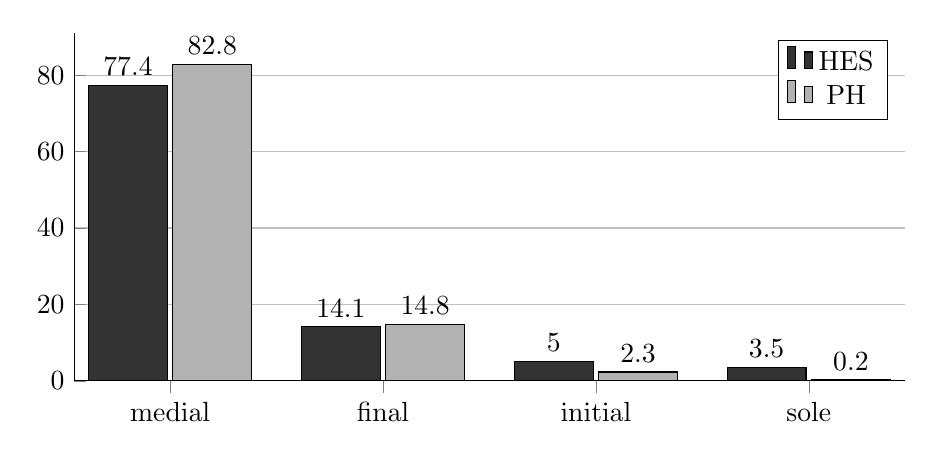
\begin{tikzpicture}
	\begin{axis}[
     axis lines*=left,
     bar width=1cm,
     enlarge x limits={0.15},
     height = 6cm,
     nodes near coords,
     symbolic x coords={medial,final,initial,sole},
     width = \textwidth,
     xtick=data,
     ybar,
     ymajorgrids=true,
     ymin=0
		]
		\addplot[black,fill=black!80] coordinates {(medial,77.4) (final,14.1) (initial,5.0) (sole,3.5)};
		\addlegendentry{HES}
		\addplot[black,fill=black!30] coordinates {(medial,82.8) (final,14.8) (initial,2.3) (sole,0.2)};
		\addlegendentry{PH}
		\end{axis}
	\end{tikzpicture}
\caption{Position of the filler in the utterance. Unclear and indeterminate examples are excluded.}
\label{fig:pakendorf:10}
\end{figure}

In the overwhelming majority of instances ({\textasciitilde}80\%) when the placeholder is repaired, the target follows immediately after the filler, although some material can intervene. This can occasionally be an explicit word search, leading to quite long distances between the placeholder and its target. The intervening material can be recycled material (e.g. the numeral ‘one’ in \REF{ex:pakendorf:12}), a prompt by an interlocutor (see \REF{ex:pakendorf:48} in \sectref{sec:pakendorf:5.1} and \REF{ex:pakendorf:58} in \sectref{sec:pakendorf:5.4}), or other parts of the placeholder phrase or the clause \REF{ex:pakendorf:13}. 


\ea \label{ex:pakendorf:12}
\gll əmən
	\textup{(0)}
	\textbf{uŋun-ma}
	\textup{(550)}
	əmən
	\uline{giβʨaːn-ma}
	βaː-ʨaː-n
	gun-ə-n…\\
    one
    {}
    \textsc{flr-acc}
    {}
    one
    roe.deer-\textsc{acc}
    kill-\textsc{pst-3sg}
    say-\textsc{nfut-3sg}\\
\glt ‘He killed a \textbf{whatchamacallit}, a \uline{deer}, he said, …’ \exsource{APN\_grindstone: 93; ID 392}
\z

\ea \label{ex:pakendorf:13}
\gll babuʃka
	smotri
	taj
	taj
	gun-ə-m
	bi
	\textup{(620)}
	\textbf{uŋunə-l}
	\textup{(0)}
	bi-si
	iʨe-kəl
	\uline{kresti-l}\\
    granny.R
    look.\textsc{imp.}R
    \textsc{dist}
    \textsc{dist}
    say-\textsc{nfut-1sg}
    \textsc{1sg}
    {}
    \textsc{flr-pl}
    {}
    \textsc{cop}-\textsc{nfut[3pl]}
    see-\textsc{imp.sg}
    cross.R-\textsc{pl}\\
\glt ‘“Granny, look there”, I say, “there are \textbf{whatchamacallits}, look, \uline{crosses}!”) \exsource{APN\_cheremsha\_brodjaga: 32; ID 300}
\z

\subsubsection{Mirroring on placeholders and recycling with targets}
\label{sec:pakendorf:4.1.1.3}
~\\
Nearly 75\% of the placeholders with an overtly expressed target fully mirror the morphology of the target, with slightly more nominal placeholders (77\%) mirroring the target morphology fully as compared to verbal placeholders (72\%). These proportions of full mirroring are considerably higher than those found in the polysynthetic Australian language Dalabon, where only 30-50\% of nominal placeholders and 5-10\% of verbal placeholders fully mirror the morphology of the target \citep{chapters/ponsonnet}. As can be seen in \figref{fig:pakendorf:11},\footnote{The label “partial”’ designates instances when the PH carries less morphology than the target and “exceeds” refers to instances when it carries more morphology than the target. The code “mismatch” was used for instances in which both PH and target carry morphology, but this is not the same (this can include occurrences where there is also a mismatch in the number of morphemes), while “bare PH” designates unmarked \textit{uŋun} standing in for a target that carries morphology.} the proportion of placeholders carrying only partially mirrored verbal morphology is twice as high as that with partially mirrored nominal morphology (24\% vs. 12\%). In Evenki, too, verbal placeholders show a higher proportion of partial mirroring than nominal placeholders \citep[211]{Klyachko2022}. As suggested by Françoise Rose and an anonymous reviewer, this higher frequency of partial mirroring with verbal placeholders might be linked to the fact that there are more verbal derivational suffixes than nominal ones, and it is the derivational suffixes that tend to be omitted from the placeholder, as detailed below.


\begin{figure}
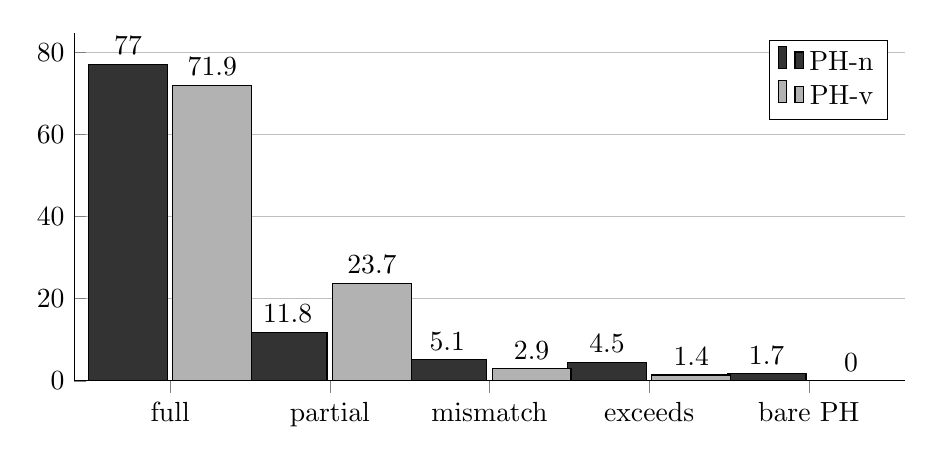
\begin{tikzpicture}
	\begin{axis}[
		ybar,
		enlarge x limits={0.15},
		ymajorgrids=true,
		xtick=data,
		axis lines*=left,
		ymin=0,
		nodes near coords,
		width = \textwidth,
		height = 6cm,
		bar width=1cm,
		symbolic x coords={full,partial,mismatch,exceeds,bare PH}
		]
		\addplot[black,fill=black!80] coordinates {(full,77.0) (partial,11.8) (mismatch,5.1) (exceeds,4.5) (bare PH,1.7)};
		\addlegendentry{PH-n}
		\addplot[black,fill=black!30] coordinates {(full,71.9) (partial,23.7) (mismatch,2.9) (exceeds,1.4) (bare PH,0)};
		\addlegendentry{PH-v}
		\end{axis}
	\end{tikzpicture}
\caption{Mirroring of target morphology on placeholders that stand in for nouns and NPs (PH-n) and verbs and VPs (PH-v) in per cent of occurrences with targets carrying “mirrorable” morphology. Instances where there is no overt target or where the placeholder and target are in Nominative case (which in Negidal is unmarked) were excluded.} 
\label{fig:pakendorf:11}
\end{figure}

The verbal placeholder does not carry any valency-changing morphology, such as the Causative suffix -\textit{βkan} or the suffix -\textit{β} that can change a transitive verb into an intransitive one \REF{ex:pakendorf:14} and an intransitive verb into a transitive one (cf. \citealt[29--31)]{AralovaPakendorf2022}, even when the target carries such morphology. This indicates that in its verbal reading \textit{uŋun} functions as an ambitransitive verb (cf. \sectref{sec:pakendorf:4.1.5}).


\ea \label{ex:pakendorf:14}
\gll ta-du
	əmən
	seːni-n
	\textup{(2350)}
	\textbf{uŋun-ə-n}
	\textup{(0)}
	\uline{loku-ʨe-β-βə-n}
	geː-n
	seːn-βa-n
	\textup{(860)}
	\textbf{uŋun-ʨaː-l}
	\textup{(3660)}
	\uline{doː-ski}
	\uline{iː-βkan-ʨaː-l}\\
    \textsc{dist-dat.ess}
    one
    ear-\textsc{3sg}
    {}
    \textsc{flr-nfut-3sg}
    {}
    hang.up-\textsc{res-val-nfut}-\textsc{3sg}
    other-\textsc{3sg}
    ear-\textsc{acc-3sg}
    {}
    \textsc{flr-pst-pl}
    {}
    inside-\textsc{advb.all}
    enter-\textsc{caus-pst-pl}\\
\glt ‘Then one ear (of the hat) \textbf{whatchamacallits}, \uline{hangs}, and they \textbf{did} \textbf{whatchamacallit}, \uline{they tucked the other one up inside}.’ \exsource{GIK\_olan: 7; ID 769-770}
\z

It is generally inflectional morphology that is mirrored: non-finite converb suffixes and the Negative Converb \REF{ex:pakendorf:15}, or finite tense\footnote{Note that I counted two examples where the placeholder carried the Future suffix -\textit{ɟa} and the target carried the suffix -\textit{ɟiŋa} as being fully mirrored, since these Future suffixes seem to occur in free variation in Negidal.} and subject markers for verbal placeholders, and case \REF{ex:pakendorf:16}, possessive, or number marking for nominal placeholders. 


\ea \label{ex:pakendorf:15}
\gll taj
	digi-la-βa
	\textup{(0)}
	\textbf{uŋun-mi}
	\textup{(1310)}
	\uline{nupki-mi}
	ela-la-βa
	nupki-mi
	o-ŋati-nen
	eːma=da
	dilkan
	\textup{(680)}
	\textbf{uŋun-a}
	\textup{(590)}
	\uline{doː-ja}
	olo-du\\
     \textsc{dist}
     four-\textsc{num(days)-acc}
     {}
     \textsc{flr-ss.cond}
     {}
     to.smoke[\textsc{tr}]-\textsc{ss.cond}
     three-\textsc{num(days)-acc}
     to.smoke[\textsc{tr}]-\textsc{ss.cond}
     \textsc{neg-deont}-\textsc{3sg}
     which=\textsc{add}
     fly
     {}
     \textsc{flr-neg.cvb}
     {}
     to.land-\textsc{neg.cvb}
     fish-\textsc{dat.ess}\\
\glt ‘\textbf{If} \textbf{you} \textbf{whatchamacallit}, \uline{if you smoke} it for four days, if you smoke it for three days, not a single fly will \textbf{whatchamacallit}, will \uline{land} on the fish.’ \exsource{DIN\_jukola: 97; ID 618-619}
\z


\ea \label{ex:pakendorf:16}
\gll eːda
	si bi
	\textup{(0)}
	\textbf{uŋun-mə-β}
	\textup{(740)}
	\uline{ɟebgɑː-βə-β}
	ɟep-ʨaː-s\\
     why
     \textsc{2sg}
     \textsc{1sg}
     {}
     \textsc{flr-acc-1sg}
     {}
     food.\textsc{Evk-acc-1sg}
     eat-\textsc{pst-2sg}\\
\glt ‘Why did you eat \textbf{my} \textbf{whatchamacallit}, \uline{my food}?’ \exsource{APK\_fox: 153; ID 193}
\z

In partial mirroring it is by and large derivational morphology that is omitted, such as the Multiplicative \REF{ex:pakendorf:17} or the Resultative (\REF{ex:pakendorf:14} above) missing from verbal placeholders, or the Diminutive suffix \REF{ex:pakendorf:18} that is omitted from nominal placeholders. Only four examples of verbal placeholders involve mirroring of aspectual morphemes, out of a total of 26 examples where the target carries such a suffix; no other derivational morphology (such as the Associated Motion suffix or the Multiplicative or Semelfactive) was found on the filler, and none of the seven evaluative morphemes found on overt nominal targets was mirrored on the placeholder. This is again similar to Evenki, where derivational morphology is omitted from the verbal placeholder \citep[211]{Klyachko2022}. Thus, the placeholder carries the inflectional morphology that is needed for syntactic integration, while morphemes that do not play a syntactic role, such as evaluatives or aspectual markers, are omitted. The filler can therefore be said to be substituting for the stem rather than the root of the target.


\ea \label{ex:pakendorf:17}
\gll a
	taj
	doldi-ʨaːki-nin
	taj
	bəjə
	oj
	uŋun-ma
	biɲag-ga
	hul-nakan
	\textup{(0)}
	\textbf{uŋunə-ji-βa-n}
	\textup{(180)}
	\uline{pəktəru-ktə-ji-βa-n}
	ŋɑːlə-l-ʨa\\
     and.R
     \textsc{dist}
     hear-\textsc{rem.pst-3sg}
     \textsc{dist}
     person
     \textsc{prox}
     \textsc{flr-acc}
     settlement\textsc{-acc}
     go-\textsc{ss.sim}
     {}
     \textsc{flr-prs.ptcp-acc-3sg}
     {}
     shoot-\textsc{mult}-\textsc{prs.ptcp-acc-3sg}
     to.fear-\textsc{inch-pst[3sg]}\\
\glt ‘And he heard that the man walking through the whatchamacallit, the village \textbf{is} \textbf{doing} \textbf{whatchamacallit}, \uline{is shooting around}, he got frightened.’ \exsource{DIN\_rok: 46; ID 685}
\z


\ea \label{ex:pakendorf:18}
\gll ɟaβa-ja-n 
	\textup{(1580)}
	\textbf{uŋun-ma}
	\textup{(360)}
	\uline{kala-ka-ʨan-ma}…\\
    grab-\textsc{nfut-3sg}
    {}
    \textsc{flr-acc}
    {}
    pot.\textsc{Evk-dim-dim-acc}\\
\glt ‘He takes \textbf{a} \textbf{whatchamacallit}, \uline{a little pot}…’ \exsource{AET\_bear: 27; ID 5}
\z

Recycling denotes the repetition of material that precedes the placeholder with the target \citep[23--25]{Podlesskaya2010}. This is quite rare in the Negidal corpus: only in about one-fifth of the examples with recyclable material in the placeholder phrase is this repeated with the target. In particular, adjuncts, direct objects, nominal modifiers \REF{ex:pakendorf:47}, demonstratives \REF{ex:pakendorf:24}, and the negative auxiliary \REF{ex:pakendorf:15} tend not to be recycled with the target. In contrast, verbs governing direct objects can be omitted or recycled with equal frequency; thus, in \REF{ex:pakendorf:19} the verb \textit{essaβun} ‘we reach’ is not repeated with the target, whereas in \REF{ex:pakendorf:20} the verb \textit{issen} ‘he plucks’ is recycled. In some instances there is recycling, but with a change in form, such as a Proximal Demonstrative being changed to a Distal Demonstrative. In the examples, the curly brackets frame the placeholder phrases containing recyclable and recycled material, where present.


\ea \label{ex:pakendorf:19}
\gll ti=tti
	\{es-sa-βun
	be…
	\textup{(0)}
	\textbf{uŋun-ma}\}
	\textup{(0)}
	\uline{mugdin-ma}\\
     like.this=\textsc{ptl}
     reach-\textsc{nfut-1pl.ex}
     \textsc{fs}
     {}
     \textsc{flr-acc}
     {}
     riverbank-\textsc{acc}\\
\glt ‘Like this we reached \textbf{whatchamacallit}, \uline{the bank}.’ \exsource{DIN\_zabludilisj: 26; ID 720}
\z


\ea \label{ex:pakendorf:20}
\gll təpu-kə-laː-jə-n
	ʨeβkan
	tik-kə-n
	gə
	\{is-se-n
	\textup{(820)}
	\textbf{uŋun-ma-n}\}
	\textup{(1020)}
	\{is-se-n
	\uline{ləpultə-βa-n\}}\\
     knock.out\textsc{{}-?sudden-smlf-nfut-3sg}
     bird(small)
     fall-\textsc{nfut-3sg}
     \textsc{dp}
     pluck-\textsc{nfut-3sg}
     {}
     \textsc{flr-acc-3sg}
     {}
     pluck-\textsc{nfut-3sg}
     feathers-\textsc{acc-3sg}\\
\glt ‘He knocked [it] out, Chevkan fell down, he plucks \textbf{whatchamacallit}, he plucks \uline{the feathers}.’ \exsource{APN\_skazka\_ptica: 22; ID 457}
\z

\subsubsection{The filler as a nominal placeholder}
\label{sec:pakendorf:4.1.4}
As a nominal placeholder, \textit{uŋun} can substitute for proper \REF{ex:pakendorf:21}, higher animate \REF{ex:pakendorf:22}, lower animate \REF{ex:pakendorf:23}, and inanimate nouns \REF{ex:pakendorf:24}. 

\ea \label{ex:pakendorf:21}
\gll oj=da
	\textup{(160)} 
	\textbf{uŋun-ŋasa}
	\textup{(0)}
	\uline{baːtur-ka-ŋasa=da}
	əmə-β-βat(-ʨe-n)\\
     \textsc{prox=add}
     {}
     \textsc{flr-dec}
     {}
     \textsc{pn-dim-dec=add}
     come-\textsc{val-hab-nfut-3sg}\\
\glt ‘And this one too, \textbf{late} \textbf{what’s-his-name}, \uline{late Batur}, he used to bring.’ \exsource{APN\_DIN\_conversation: 39; ID 318}
\z


\ea \label{ex:pakendorf:22}
\gll taj
	boa
	baja-sal
	biɲagi-tin
	boagda-du-n
	iʨe-t-ʨe-n
	iʨe-je-n
	\textup{(1050)}
	\textbf{uŋun-ma}
	\textup{(1330)}
	\uline{olgin-ma}\\
     \textsc{dist}
     \textsc{fs}
     rich-\textsc{pl.hum}
     settlement-\textsc{3pl}
     yard-\textsc{dat.ess-3sg}
     see-\textsc{tam2-nfut-3sg}
     see-\textsc{nfut-3sg}
     {}
     \textsc{flr-acc}
     {}
     pig-\textsc{acc}\\
\glt ‘In the settlement of those rich people he saw \textbf{a} \textbf{whatchamacallit}, \uline{a pig} in the yard.’ \exsource{TIN\_swine: 61; ID 879}
\z


\ea \label{ex:pakendorf:23}
\gll gə
	taj
	kuhi-rə
	\textup{(0)}
	\textbf{taj}
	\textbf{uŋu-l-ɟi}
	\textup{(610)}
	\uline{taj}
	\uline{dilka-l-ɟi}\\
     \textsc{dp}
     \textsc{dist}
     to.fight.\textsc{Evk}-\textsc{nfut.Evk[3pl]}
     {}
     \textsc{dist}
     \textsc{flr-pl-ins}
     {}
     \textsc{dist}
     fly-\textsc{pl-ins}\\
\glt ‘So they are fighting with \textbf{those} \textbf{whatchamacallits}, \uline{those flies}.’ \exsource{APN\_koldekan: 94; ID 429}
\z

\ea \label{ex:pakendorf:24}
\gll nu
	ʨindɑkaː-ʨan
	taj
	\textup{(0)}
	\textbf{uŋun-duli-n}
	\textup{(570)}
	\uline{soːna-li-tin}
	iː-je-n=da tadu\\
     \textsc{ptl.}R
     little.bird-\textsc{dim}
     \textsc{dist}
     {}
     \textsc{flr-prol-3sg}
     {}
     smoke.hole.\textsc{Evk}-\textsc{prol-3pl}
     enter-\textsc{nfut-3sg=add}
     there\\
\glt ‘Well, the bird (entered) \textbf{via} \textbf{whatchamacallit}, it entered there \uline{via the smoke hole}.’ \exsource{APK\_1chindakan: 81-82; ID 154}
\z

The filler can also stand in for different types of NPs (cf. \citealt[263]{Schegloff1979}; this is also found in the Tungusic language Even \citep{Matić2008} and in the Nakh-Daghestanian languages Udi and Aghul (\citealt[101]{GanenkovGanenkov2010})): attributive, conjoined \REF{ex:pakendorf:25}, possessive, and NPs with a relational noun functioning as a postposition \REF{ex:pakendorf:26}. The attributive NPs can be quite elaborate and include relative clauses, which in Negidal are participial \REF{ex:pakendorf:27}.


\ea \label{ex:pakendorf:25}
\gll ɟe
	taj
	hətəkɑːsi-l-ʨaː-du-n
	taj
	uj
	geda-ʨaːki-nin
	\textup{(0)}
	\textbf{uŋun}
	\textup{(0)}
	\uline{ʨeβkaː-ʨa-l}
	\uline{siŋəjə-ʨa-l}
	ɟe uŋun-duki-n
	tətʨanŋa-duki-n
	hətəkən-ə\\
     \textsc{interj}
     \textsc{dist}
     jump[\textsc{iter]-inch-pst.ptcp-dat.ess-3sg}
     \textsc{dist}
     recently
     shove.into-\textsc{rem.ptcp-3sg}
     {}
     \textsc{flr}
     {}
     bird-\textsc{dim-pl}
     mouse-\textsc{dim-pl}
     \textsc{interj}
     \textsc{flr-abl-3sg}
     clothing-\textsc{abl-3sg}
     jump[\textsc{smlf}]-\textsc{nfut[3pl]}\\
\glt ‘When he started jumping, those \textbf{whatchamacallit}, \uline{little birds and mice}, which he had hidden, jumped out of whatchamacallit, out of his clothes.’ \exsource{APK\_fox: 140; ID 184}
\z


\ea \label{ex:pakendorf:26}
\gll goja-βa
	tigdə-ŋəsə-n
	tukti-ʨaː
	\textup{(0)}
	\textbf{uŋun-tiki}
	\textup{(0)}
	\uline{koridor-βi}
	\uline{ugi-da-tki-n}\\
     distance-\textsc{acc}
     rain-\textsc{vs.sim-3sg}
     ascend-\textsc{pst[3sg]}
     {}
     \textsc{flr-all}
     {}
     lean.to.R-\textsc{prfl.sg}
     top-\textsc{side-all-3sg}\\
\glt ‘When it rained for a long time he climbed up \textbf{to} \textbf{whatchamacallit}, \uline{on top of his lean-to}.’ \exsource{APN\_DIN\_weather: 18; ID 371}
\z

\ea \label{ex:pakendorf:27}
\gll noŋan
	sinə-βə
	gunə
	gun-ə-n
	taj
	\textup{(0)}
	\textbf{uŋun-ma}
	\textup{(3030)}
	\uline{vorona-βa}
	\uline{atikaŋi-n}
	\uline{noda-ʨa-βa}
	aja-ma-t
	ulguʨaːn-da-s\\
     \textsc{3sg}
     \textsc{2sg.obl-acc}
     \textsc{fs}
     say-\textsc{nfut-3sg}
     \textsc{dist}
     {}
     \textsc{flr-acc}
     {}
     crow.R-\textsc{acc}
     wife\textsc{-3sg}
     throw-\textsc{pst.ptcp-acc}
     good-\textsc{ints-advr}
     tell-\textsc{vs.purp-2sg}\\
\glt ‘She is asking you to tell nicely \textbf{about} \textbf{whatchamacallit} \uline{about the crow whose wife left him}.’ \exsource{APN\_birds: 98; ID 293}
\z

It can also substitute for adjectives in predicative position \REF{ex:pakendorf:28}; however, only two such examples occur in the corpus. Note that the Evenki filler \textit{aŋi}/\textit{aŋə} can also stand in for predicative adjectives, as shown by an example provided by \citet[207, her ex. (12)]{Klyachko2022}.




\ea \label{ex:pakendorf:28}
\gll noŋan
	bi-ʨa-n
	so
	\textup{(0)}
	\textbf{uŋun}
	\textup{(340)}
	\uline{ujimkun}
	i
	muː-du
	ɟaβu-ʨa-ja-n\\
     \textsc{3sg}
     \textsc{cop-pst-3sg}
     very
     {}
     \textsc{flr}
     {}
     light
     and.R
     water-\textsc{dat.ess}
     take-\textsc{res-nfut-3sg}\\
\glt ‘It was very \textbf{whatchamacallit}, \uline{light} and floated upon the water.’ \exsource{AVK\_crossing\_stream: 105; ID 492}
\z

The target is often provided subsequently (see for instance (\ref{ex:pakendorf:25})-(\ref{ex:pakendorf:28})), but this need not be the case – as mentioned in \sectref{sec:pakendorf:4.1.1.1}, the target is left unspecified in nearly 30\% of the examples with a nominal placeholder. Such omission frequently occurs because the target is obvious from the speech situation, as in \REF{ex:pakendorf:29} taken from a procedural text about hide preparation: this was uttered at the moment when the speaker turned to pick up a particular tool. Occasionally, the target is described with a clause, such as the headless relative clause in \REF{ex:pakendorf:30}. Note that in this example the speaker finally resorts to using the Russian lexeme that she seems to have wanted to avoid, since she cannot come up with a Negidal equivalent. There is no indication that \textit{uŋun} can have a vague, generic meaning rather than standing in for a particular noun or noun phrase that is eluding the speaker.


\ea \label{ex:pakendorf:29}
\gll ɟaβa-m
	geː
	\textup{(590)}
	\textbf{uŋun-ma}
	\textup{(590)}\\
     take[\textsc{nfut]-1sg}
     other
     {}
     \textsc{flr-acc}
     {}\\
\glt ‘Then I take the next \textbf{whatchamacallit} (instrument).’ \exsource{DIN\_preparing\_hide: 157; ID 661}
\z

\ea \label{ex:pakendorf:30}
\gll
	ulguma-ja-n
	min-du
	nɑː-ɟə-m
	taj
	əŋun…
	\textup{(0)}
	\textbf{uŋun-mi}
	\textbf{doː-du-n}
	\textup{(570)}
	\uline{taj}
	\uline{olo-ŋi-n}
	\uline{nɑː-kʨi-ji-n}
	\uline{doː-du-n}
	\textup{(830)}
	\textbf{uŋun-du-j}
	\textup{(470)}
	\uline{kul-du-j}\\
     ask-\textsc{nfut-3sg} \textsc{1sg.obl-dat.ess} put-\textsc{q.fut-1sg} \textsc{dist} \textsc{fs} {} \textsc{flr-prfl.sg} inside-\textsc{dat.ess-3sg} {} \textsc{dist} fish-\textsc{poss-3sg} put-\textsc{dur}-\textsc{prs.ptcp-3sg} inside-\textsc{dat.ess-3sg} {} \textsc{flr-dat.ess-prfl.sg} {} sack\textsc{{}-dat.ess-prfl.sg}\\
\glt ‘She asks me whether to put it \textbf{into} \textbf{the} \textbf{whatchamacallit} (lit. She asks me “should I put it into my whatchamacallit”), \uline{into that where she puts the fish}, \textbf{in} \textbf{the} \textbf{whatchamacallit}, \uline{in the sack}.’ \exsource{GIK\_shuka: 38-39; ID 787-788}
\z

There are furthermore three examples in which the filler appears to be standing in for direct speech \REF{ex:pakendorf:31}, as shown by prosody and the fact that in two examples the fillers were translated as speech complements,\footnote{I reflect this in the translation of \REF{ex:pakendorf:31} by exceptionally not translating the placeholder as ‘whatchamacallit’.} indicating that our consultant interpreted them as holding the place for direct speech utterances. Furthermore, \textit{uŋun} is marked with the Accusative case expected for the complement of the speech verb in example \REF{ex:pakendorf:31}. Unfortunately, two of these examples come from one of the old digitized tape recordings, so that the extraction of the pitch contour in Praat is full of errors. Nevertheless, a rise in pitch on the first syllable can clearly be identified in Praat (\figref{fig:pakendorf:12}); this differs from the prosody of hesitative uses of \textit{uŋun}, justifying the interpretation that \textit{uŋun} has a placeholder function here. 


\ea \label{ex:pakendorf:31}
\gll minə-βə
	gun-ʨa-n
	\textup{(820)}
	\textbf{uŋun-ma}
	\textup{(1570)}
	\uline{kaʨikan-ma-s}
	\uline{bi}
	\uline{ɟepu-βka-ŋta…}\\
     \textsc{1sg.obl-acc}
     say-\textsc{pst-3sg}
     {}
     \textsc{flr-acc}
     {}
     puppy-\textsc{acc-2sg}
     \textsc{1sg}
     eat-\textsc{caus-hort.sg}\\
\glt ‘It said \textbf{this} to me: “\uline{Let me feed your puppy,…}”’ \exsource{APK\_1chindakan: 62-63; ID 153}
\z

\begin{figure}
\includegraphics[clip, trim=0cm 5.9cm 0cm 2.5cm, width=\textwidth]{Fig12_153.pdf}
\caption{Waveform and pitch contour of example \REF{ex:pakendorf:31}}
\label{fig:pakendorf:12}
\end{figure}

Such uses of the filler are also attested in Evenki, but  \citet[207]{Klyachko2022} analyses them as instances of hesitative uses rather than as placeholder.

\subsubsection{The filler as verbal placeholder}
\label{sec:pakendorf:4.1.5}
As a verbal placeholder, \textit{uŋun} can stand in for both intransitive \REF{ex:pakendorf:32} and transitive \REF{ex:pakendorf:33} verbs without taking any additional valency-changing morphology, similar to the Manambu placeholder verb \textit{məgi}- (\citealt[399--400, 575]{Aikhenvald2008}). This implies that \textit{uŋun} can be analysed as an ambitransitive verb – which explains the lack of valency-changing morphology on the filler even when the target carries such morphology, as mentioned above (\sectref{sec:pakendorf:4.1.1.3}). The filler can also stand in for a VP (see the coding definitions for details on how these were identified), substituting for the verb plus adjunct (\ref{ex:pakendorf:8}, \ref{ex:pakendorf:14}) or direct object.


\ea \label{ex:pakendorf:32}
\gll atikaː-sal
	gə təgə-dgi-jaːn
	\textup{(890)}
	\textbf{uŋu-l-ʨaː-l}
	\textup{(0)}
	\uline{məjgɑː-l-ʨaː-l}
	gun-ə\\
	old.woman-\textsc{pl.hum}
	\textsc{dp}
	sit.down-\textsc{rep-ss.ant}
	{}
	\textsc{flr-inch-pst-pl}
	{}
	think-\textsc{inch-pst-pl}
	say-\textsc{nfut[3pl]}\\
\glt ‘The old women, having sat down, \textbf{started} \textbf{to} \textbf{whatchamacallit}, \uline{started to think}, they say:…’ \exsource{GIK\_olan: 23; ID 768}
\z


\ea \label{ex:pakendorf:33}
\gll tadukin
	aja
	ajag
	ajaŋis-saːn
	opuška-ja-n
	\textup{(0)}
	\textbf{uŋun-ə-s}
	\textup{(280)}
	\uline{tulə-s}\\
	then good \textsc{fs} adjust.properly-\textsc{ss.ant} trimming.R-\textsc{dest-3sg} {} \textsc{flr-nfut-2sg} {} attach\textsc{[nfut]-2sg}\\
\glt ‘Then, having adjusted (the centre) properly \textbf{you} \textbf{whatchamacallit}, \uline{you add} the trimming.’ \exsource{DIN\_duck\_heads: 75; ID 577}
\z

However, even though as a verb \textit{uŋun} is mostly used as a placeholder (e.g. \REF{ex:pakendorf:6}, \REF{ex:pakendorf:14}, \REF{ex:pakendorf:15}, \REF{ex:pakendorf:17} above), both with and without an overt target, there are also several instances where it functions as a generic action verb.\footnote{In \sectref{sec:pakendorf:4.1.1.1} to \sectref{sec:pakendorf:4.1.1.3} all tokens of \textit{uŋun} carrying verbal morphology were included in the counts for verbal placeholder.} These uses probably account in part for the very high frequency (50\%) of verbally used \textit{uŋun} without an overt target (\sectref{sec:pakendorf:4.1.1.1}). It can refer to a general, unspecified action (‘do’), as in \REF{ex:pakendorf:34}, which is taken from a narrative about a game in which the loser has to fulfill the wish of the winner. Here, the loser is asking the winner what it is he should do for her, i.e. the reference is clearly to an as yet unspecified action. The filler can also be used deictically (mostly accompanied by the manner demonstrative \textit{tiː} ‘like this’), referring anaphorically to what was said in the preceding discourse \REF{ex:pakendorf:35} or exophorically to what is being done in the speech situation \REF{ex:pakendorf:36}.\footnote{I refrain from adding pause lengths to this example, since the pauses were the result of the demonstration and are hence not indicative of any form of disfluency.} Such examples with exophoric meaning are mostly found in the procedural texts, and in the accompanying video one can see that the filler is accompanied by the appropriate action (\figref{fig:pakendorf:13}). 


\ea \label{ex:pakendorf:34}
\gll gə eːkun-ma \textup{(0)} \textbf{uŋun-ŋati-β} \textup{(0)} gun-ə-n\\
\textsc{dp} what-\textsc{acc} {} \textsc{flr-deont-1sg} {} say-\textsc{nfut-3sg}\\
\glt ‘“Well, what \textbf{shall} \textbf{I} \textbf{do} (for you)?”, he says.’ \exsource{DIN\_games: 34; ID 594}
\z

\ea \label{ex:pakendorf:35}
\gll a
	osi
	ti-kan
	\textup{(0)}
	\textbf{o-ta-s}
	\textbf{uŋun-a}\\
	and.R
	now
	like.this-\textsc{dim}
	{}
	\textsc{neg-neg.fut-2sg}
	\textsc{flr-neg.cvb}\\
\glt \{In the past we fished as much as [we needed]. There was a little house like that up high [on piles] and there we put the dried fish so that it would last all year for us and for our dogs.\} ‘But now \textbf{you} \textbf{can't} \textbf{do} like that.’ \exsource{AET\_village\_life: 90; ID 135}
\z


\ea \label{ex:pakendorf:36}
\gll saː-ŋati-s olgo-ʨa-βa-n \textbf{tiː} \textbf{uŋun-e-ki-s} \textbf{tiː} \textbf{uŋun-gi-je-ki-s} oː-ŋati-nin nəptə-mdi\\
know-\textsc{deont-2sg} dry.out\textsc{[intr]-pst.ptcp-acc-3sg} like.this \textsc{flr-nfut-cond-2sg} like.this \textsc{flr-rep-nfut-cond-2sg} become-\textsc{deont-3sg} smooth-\textsc{ints.adj}\\
\glt ‘You will know that it's dry if, when \textbf{you} \textbf{do} \textbf{like} \textbf{this} and \textbf{when} \textbf{you} \textbf{do} \textbf{it} \textbf{again}, it straightens out.’ \exsource{DIN\_preparing\_hide: 185; ID 662-663}
\z


\begin{figure}
\begin{tabularx}{\textwidth}{XX}
\includegraphics[width=0.4\textwidth]{Fig13_662_V1.png} & 
\includegraphics[width=0.4\textwidth]{Fig13_662_V2.png}
\\
\textit{tiː uŋunekis} & \textit{tiː uŋungijekis}
\end{tabularx}
\caption{Two still frames taken from the video that illustrate the rolling up and unrolling gestures that accompany the tokens of \textit{uŋun} in example \REF{ex:pakendorf:36}}
\label{fig:pakendorf:13}
\end{figure}

Example \REF{ex:pakendorf:36} is taken from a recording in which the speaker explained and demonstrated how the Negidals prepare elk hide. Here, she shows how you can judge whether you have scraped off all the moisture by rolling it up (‘when you do like this’) and then unrolling it again (‘you do it again’ – with the refactive suffix \textit{–(d)gi}).

There are also examples in which \textit{uŋun} is used not as a placeholder for a target that eludes the speaker nor with anaphoric reference, but to substitute for a verb that was used in the immediately preceding context \REF{ex:pakendorf:37}.\footnote{This is an example without a sound file, hence the pause duration cannot be established.} Such uses of the filler have also been identified for Northern Pastaza Kichwa, where \cite{chapters/rice} terms them ‘resumptive pro-verbs’. The function of such resumptive uses of the filler is unclear, but it is unlikely to be a problem with the planning or execution of speech. Nor is it likely to be the avoidance of repetition of the lexical verb, as shown by the fact that the sentence following \REF{ex:pakendorf:37} contains three tokens of the verb ‘eat’.

\ea \label{ex:pakendorf:37}
\gll taj bəjun \uline{tiː} \uline{ɟepu-βki}, ɟaɟa \textbf{tiː} \textbf{ə-βki} \textbf{uŋun-a}\\
\textsc{dist} elk like.this eat-\textsc{hab.ptcp} bear[\textsc{euph}] like.this \textsc{neg}-\textsc{hab.ptcp} \textsc{flr-neg.cvb}\\
\glt ‘An elk \uline{eats like this}, but not a bear. (Lit. An elk eats like this, a bear \textbf{doesn’t} \textbf{do}). \{Why would a bear eat a tree? A bear eats berries, it eats nuts.\}’ \exsource{APN\_DIN\_galigda: 210; ID 345}
\z

In the verbal uses in which it does not function as a placeholder, \textit{uŋun} partly overlaps with the generic action verb \textit{ɲeko}{}- ‘do’. Next to its use to refer to unspecified actions \REF{ex:pakendorf:38}, sometimes with anaphoric \REF{ex:pakendorf:39} or exophoric reference, \textit{ɲeko}{}- is used as a light verb with ideophones \REF{ex:pakendorf:40}. 


\ea \label{ex:pakendorf:38}
\gll eːkun-ma \textbf{ɲeko-ŋaːti-}s\\
what-\textsc{acc} do-\textsc{deont-2sg}\\
\glt ‘What are \textbf{you} \textbf{going} \textbf{to} \textbf{do}?’ \exsource{GIK\_1belekakta: 1}
\z


\ea \label{ex:pakendorf:39}
\gll \textbf{tiː} \textbf{ɲeko-jaːn} mani-n juː-ja-n ŋənə-jə-n\\
like.this do-\textsc{ss.ant} self-\textsc{3sg} exit-\textsc{nfut-3sg} go-\textsc{nfut-3sg}\\
\glt ‘\textbf{Having} \textbf{done} \textbf{this} he himself exits and leaves.’ \exsource{DIN\_girl\_devil: 77}
\z


\ea \label{ex:pakendorf:40}
\gll … araj taj-du-n uŋun-du-n həjə-du-n eːkun=ka \textbf{kopeːr} \textbf{kopeːr} \textbf{ɲeko-jə-n}\\
     … \textsc{restr.Evk} \textsc{dist-dat.ess-3sg} \textsc{flr-dat.ess-3sg} bottom-\textsc{dat.ess}{}-\textsc{3sg} what=\textsc{foc} \textsc{ideo} \textsc{ideo} do-\textsc{nfut-3sg}\\
\glt ‘… only something at the bottom [of the sack] is rattling (lit. \textbf{does} \textbf{koper-koper}).’ \exsource{APK\_fox: 107}
\z

The generic action verb \textit{ɲeko}- is furthermore frequently used as an auxiliary in analytical constructions with a prospective reading, that is, in constructions with a reading of imminence, often with a nuance of intention or desire (see \citealt{Matić2017} for a description of this construction in Negidal’s sister Even). This construction consists of the lexical verb in the Reflexive-marked Purposive Converb form -\textit{da-j} (\textsc{sg}) or -\textit{da-βaj} (\textsc{pl}) with \textit{ɲeko}- acting as auxiliary \REF{ex:pakendorf:41}. There are three examples in the corpus where \textit{uŋun} takes the place of the auxiliary \textit{ɲeko}- in such prospective constructions, e.g. \REF{ex:pakendorf:42}, but no examples where \textit{uŋun} functions as a light verb with ideophones. 


\ea \label{ex:pakendorf:41}
\gll iʨe-t-ʨe siβu-ŋi-tin ələ \textbf{təgə-da-j} \textbf{ɲeko-l-ʨaː}\\
     see-\textsc{tam2-nfut[3pl]} sun-\textsc{poss-3pl} already sit.down-\textsc{vs.purp}{}-\textsc{prfl.sg} do-\textsc{inch-pst[3sg]}\\
\glt ‘They look: the sun \textbf{is} \textbf{about} \textbf{to} \textbf{go} \textbf{down}. (lit. is about to sit down)’ \exsource{GIK\_kljukva: 16}
\z

\ea \label{ex:pakendorf:42}
\gll \textbf{puktəran-da-j}
	ələ
	\textup{(0)}
	\textbf{uŋun-ʨa-n}, 
	\textup{(0)} 
	...\\
    shoot-\textsc{vs.purp-prfl.sg}
    already
    {}
    \textsc{flr-pst-3sg}
    {}
    {}\\
\glt ‘He was already \textbf{about} \textbf{to} \textbf{shoot}…’ \exsource{AET\_bear: 20; ID 4}
\z

However, while the filler overlaps partly with \textit{ɲeko}{}- in its use as a generic verb, \textit{uŋun} is the only verbal placeholder: there are no examples in the corpus in which \textit{ɲeko}{}- substitutes for another verb.  

In three examples in the corpus, which were all uttered by the same speaker, the filler seems to be substituting not for a verb (phrase), but for an independent clause.  In two examples, one of which is shown here \REF{ex:pakendorf:43}, it is a 3\textsc{pl} Non-Future tense-marked filler that refers to the following clause, as shown by the prosody, which is clearly that of a syntactically integrated verb and not a hesitative (\figref{fig:pakendorf:14}), and the translation provided by our consultant, which included the filler. 

\ea \label{ex:pakendorf:43}
\gll gə
	taj
	bi-ɟe-mneːn
	\textup{(0)}
	\textbf{uŋun-ə}
	\textup{(860)}
	\uline{əmɑːʨin-a-βaj}
	\uline{oː-naː-ʨa-l}
	\uline{diː-ski}\\
     \textsc{dp}
     \textsc{dist}
     live-\textsc{dur-ss.dur}
     {}
     \textsc{flr-nfut[3pl]}
     {}
     birchbark.boat-\textsc{dest}-\textsc{prfl.pl}
     make-\textsc{am-pst-pl}
     taiga-\textsc{advb.all}\\
\glt ‘Well, living like that \textbf{they} \textbf{do} \textbf{something}, \uline{they went to the forest to make a boat for themselves}.’ \exsource{APN\_two\_sisters: 4-5; ID 485}
\z

\begin{figure}
\includegraphics[clip, trim=0cm 5.9cm 0cm 2.5cm, width=\textwidth]{Fig14_485.pdf}
\caption{Waveform and pitch contour of example \REF{ex:pakendorf:43}}
\label{fig:pakendorf:14}
\end{figure}

In these examples, \textit{uŋun} is translated with ‘do (something)’ ({что}-{то} {делают}), similar to its use with anaphoric or exophoric reference, but here the reference is cataphoric, to an event that has not yet been mentioned by the speaker. Whether this has a particular discourse function or is merely a means to gain time to gather one’s thoughts cannot be judged given the small number of examples.

In the third example \REF{ex:pakendorf:44}, the filler is unmarked, yet prosodically it can be identified as a placeholder, since its pitch does not drop down to the level often found for hesitatives (\figref{fig:pakendorf:15}). Furthermore, it was translated as the complement of ‘see’ by our consultant. The substituted clause is finite and thus grammatically not a complement clause (which in Negidal would take an Accusative-marked participial predicate), but the context makes it clear that what the speaker sees is the boat coming.

\ea \label{ex:pakendorf:44}
\gll iʨe-je-βun
	\textup{(0)}
	\textbf{uŋun}
	\textup{(0)}
	\uline{əmən}
	\uline{oŋoʨo-kan}
	\uline{əmə-jə-n}\\
     see-\textsc{nfut-1pl.ex}
     {}
     \textsc{flr}
     {}
     one
     boat.E\textsc{vk}-\textsc{dim}
     \textsc{come-nfut-3sg}\\
\glt ‘\{We went there. Going we saw.\} We saw \textbf{something}, \uline{a boat is coming}.’ \exsource{APN\_anecdotes: 16; ID 275}
\z

\begin{figure}
\includegraphics[clip, trim=0cm 5.9cm 0cm 2.5cm, width=\textwidth]{Fig15_275.pdf}
\caption{Waveform and pitch contour of example \REF{ex:pakendorf:44}}
\label{fig:pakendorf:15}
\end{figure}

To summarize what was said in \sectref{sec:pakendorf:4.1}, the Negidal filler \textit{uŋun} occurs with high frequency in spoken discourse, with the placeholder strategy dominating over the hesitative strategy; however, targets are frequently left unexpressed. It takes the place of nouns and verbs with equal frequency and thus goes against the cross-linguistic tendency for placeholders to occur more commonly with nominal than with verbal targets \citep[13]{Podlesskaya2010}. While the filler carrying verbal morphology often has a reading of a generic action verb, \textit{uŋun} used as a noun does not seem to have any vague or generic meaning. In addition to substituting for nouns and verbs the filler can also stand in for clauses and direct speech, although this is very rare in the data and restricted to the two speakers who were born before 1925. This is not the only inter-speaker difference in use of the filler, as will be addressed in the following section.

\subsection{Differences in use of \textit{uŋun} between speakers}
\label{sec:pakendorf:4.2}

As can be seen in \figref{fig:pakendorf:16}, the frequency of the filler varies considerably across speakers. Such inter-speaker variability has also been found for markers of disfluency in German women \citep{BraunBraun2023}, and for the use of placeholders in Kalamang \citep{chapters/visser} and Besemah \citep{chapters/mcdonnell_billings} spoken in Indonesia, Kolyma Yukaghir spoken in Siberia \citep{chapters/ventayol_boada}, and among three speakers of the endangered Australian language Dalabon \citep{chapters/ponsonnet}.

\begin{figure}
\begin{tikzpicture}
	\begin{axis}[
		ybar,
		enlarge x limits={0.15},
		ymajorgrids=true,
		xtick=data,
		axis lines*=left,
		ymin=0,
		nodes near coords,
		width = \textwidth,
		height = 6cm,
		bar width=1cm,
		symbolic x coords={GIKlju (1),LIO (4),AVK (34),AET (138),TIN (45),GIK (137),DIN (185),APN (225),APK (112)},
        x tick label style={text width=1cm,align=center}
        ]
		\addplot[black,fill=black!80]
		coordinates {(GIKlju (1),3.2) (LIO (4),6.6) (AVK (34),35.4) (AET (138),54.7) (TIN (45),5.8) (GIK (137),16.1) (DIN (185),6.4) (APN (225),10.3) (APK (112),26.7)};
		\path let \p1=(current axis.west), \p2=(axis cs:{LIO (4)},11.6) in coordinate (point1) at (\x1,\y2);
		\path let \p1=(current axis.east),
		\p2=(axis cs:{LIO (4)},11.6) in coordinate (point2) at (\x1,\y2);
		\draw [dashed,black!80] (point1) -- (point2);
	\end{axis}
	\end{tikzpicture}
\caption{Frequency of use of \textit{uŋun} by speaker, normalized to 1000 words. Speaker ID’s are arranged in order of increasing proficiency, and the absolute number of \textit{uŋun} they produced is indicated in brackets. The dashed line indicates the corpus average (11.6 per thousand words).}
\label{fig:pakendorf:16}
\end{figure}

Interestingly, there is no linear correlation with the proficiency of the speakers (\figref{fig:pakendorf:16}). It is likely that the two speakers who use the filler most, namely AVK and AET, do so because they are relatively weak and insecure speakers (\citealt{PakendorfAralova2018}). The influence of language proficiency on the rate of filler use has also been demonstrated for Evenki \citep[213--214]{Klyachko2022} and been observed for filled pauses in general (\citealt[220]{KosmalaCrible2022}). In this context it is a bit surprising that the two weakest speakers, GIKlju and LIO, produce hardly any \textit{uŋun}. However, for her own contribution to the corpus GIKlju only read a prepared text, which not unsurprisingly contains no fillers; the one filler she did produce was while trying to ask AVK a question in Negidal during the recording of the latter’s narrative. With respect to LIO, it might be that she was actually more proficient in Negidal than the few very hesitant narratives recorded with her led us to believe – this is indicated by a fluent spontaneous interaction with her mother which was recorded when she served as an interlocutor. Rather harder to explain is the relatively high frequency of use of the filler by the only male speaker, APK, who is said to have had an “excellent knowledge of the language” (\citealt[227]{KhasanovaKhasanova2003}, my translation). Possibly his above-average use of the filler is due to a certain pressure to narrate folktales in a specific way using particular terms and phrases (\citealt[233--234]{KhasanovaKhasanova2003}). This might have induced him to hesitate frequently (see \figref{fig:pakendorf:18} below) while he remembered necessary details.

An alternative explanation for the inter-speaker variability in frequency of filler use, suggested by an anonymous reviewer, is the impact of differences in Negidal practice among different speakers. Since Negidal is hardly used in everyday life anymore, the speakers who contributed to the corpus would have gained fluency over the period they worked with the recording linguists. Speakers who did not contribute much text would have remained relatively rusty in Negidal, and hence resorted to the filler a lot while searching for forgotten words, while speakers who produced more recordings would have acquired practice speaking it for the linguists and hence produced less fillers overall. However, a breakdown of the frequency of filler use by year for the three speakers (APN, DIN, and GIK) for which the corpus contains recordings made over several years (\figref{fig:pakendorf:17}) does not show the linear decrease over time that would be expected if language practice were the only factor at play. It is true that there is a drastic drop in occurrence of the filler in GIK’s production between 2005 and 2006, which might indicate some form of habituation. However, based on my own work with GIK, I think it is more likely diffidence rather than rustiness that made her hesitate, with the drop in filler use in later years being due to her increasing familiarity with the recording linguists.   

\begin{figure}
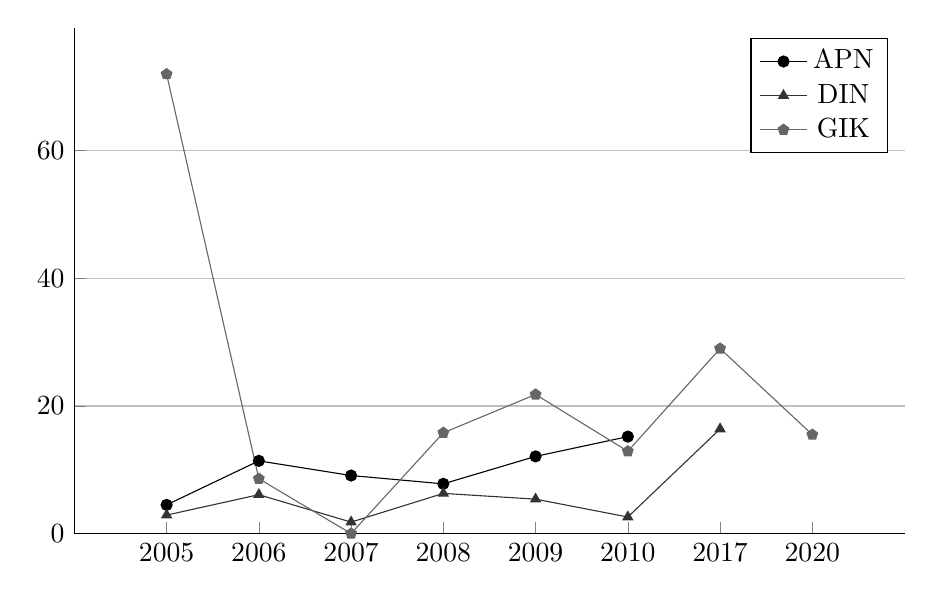
\begin{tikzpicture}
	\begin{axis}[
		xtick=data,
		axis lines*=left,
        width = \textwidth,
		height = 8cm,
        ymajorgrids=true,
	    xmin=0, xmax=180,
	    ymin=0,
	    xtick={20,40,60,80,100,120,140,160},
	    xticklabels={2005,2006,2007,2008,2009,2010,2017,2020},
	            ]
	\addplot[mark=*,black] plot coordinates {
	    (20,4.5)
	    (40,11.4)
	    (60,9.1)
	    (80,7.8)
	    (100,12.1)
	    (120,15.2)
	};
	\addlegendentry{APN}

	\addplot[color=black!80,mark=triangle*]
	    plot coordinates {
	    (20,2.9)
	    (40,6.1)
	    (60,1.8)
	    (80,6.3)
	    (100,5.4)
	    (120,2.6)
	    (140,16.4)
	    };
	\addlegendentry{DIN}

	\addplot[color=black!60,mark=pentagon*]
	    plot coordinates {
 		(20,72.0)
	    (40,8.6)
	    (60,0.0)
	    (80,15.8)
	    (100,21.8)
	    (120,12.9)
	    (140,29.0)
	    (160,15.5)
	    };
	\addlegendentry{GIK}
	\end{axis}
\end{tikzpicture}
\caption{Frequency of filler use (per 1000 words) by year of recording for the speakers APN, DIN, and GIK. These are the only speakers for whom the corpus contains recordings made over several years as documented by metadata.}
\label{fig:pakendorf:17}
\end{figure}

Speakers do not only differ in the frequency with which they use fillers, but also in their choice of hesitatives vs. placeholders (cf. \cite{chapters/visser} for a similar finding for the Papuan language Kalamang, albeit taking into account also the hesitative ‘uh(m)’, which is excluded in my study). DIN makes very little use of \textit{uŋun} as a hesitative, with only 10\% of her tokens falling into this category (\figref{fig:pakendorf:18}); this contrasts strikingly with AET, nearly half of whose tokens of the filler (46\%) are hesitatives. 

\begin{figure}
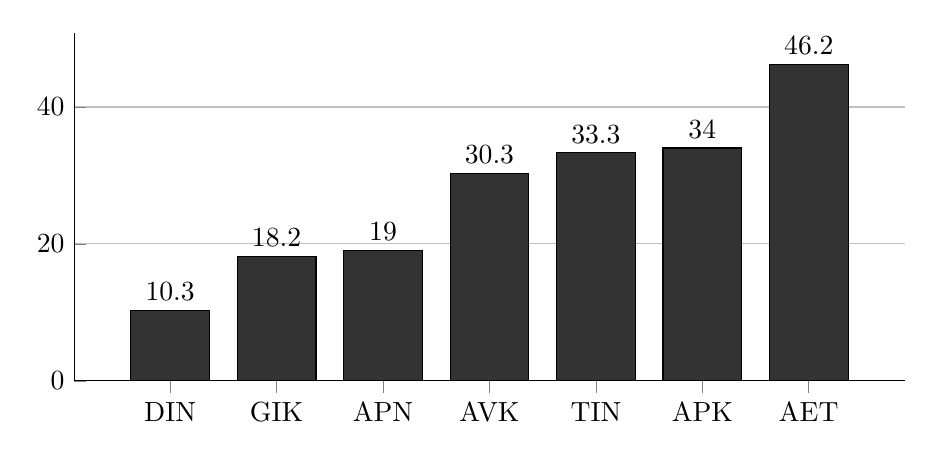
\begin{tikzpicture}
	\begin{axis}[
		ybar,
		enlarge x limits={0.15},
		ymajorgrids=true,
		xtick=data,
		axis lines*=left,
		ymin=0,
		nodes near coords,
		width = \textwidth,
		height = 6cm,
		bar width=1cm,
		symbolic x coords={DIN,GIK,APN,AVK,TIN,APK,AET}
		]
		\addplot[black,fill=black!80]
		coordinates {(DIN,10.3) (GIK,18.2) (APN,19.0) (AVK,30.3) (TIN,33.3) (APK,34.0) (AET,46.2)};
	\end{axis}
	\end{tikzpicture}
\caption{Proportion (in per cent) of hesitative use of filler tokens produced by individual speakers, arranged by increasing frequency of hesitatives. Unclear and indeterminate tokens were excluded from the total count. Since GIKlju and LIO produced hardly any fillers, they are omitted from the figure.}
\label{fig:pakendorf:18}
\end{figure}

This difference – which results in a difference between fluent vs. hesitant speech – can probably be partly explained by differences in language proficiency, since DIN, GIK, and APN are relatively proficient speakers, while AET is one of the speakers with the least active use of Negidal and hence lacks proficiency. In addition, the pressure to produce narratives in a particular way and to speak “proper” Negidal might also have an impact on the amount of hesitative vs. placeholder uses of the filler. Thus, as mentioned above, the fact that APK, a proficient speaker, uses the filler as a hesitative rather than placeholder in 35\% of his tokens might be due to the pressure to narrate fairy tales in a precise way following particular conventions. This could have increased his hesitancy without increasing the need to search for lexemes. Similar pressures can explain the relatively high frequency of hesitative uses for TIN (33\%) and AVK (30\%): as mentioned in \sectref{sec:pakendorf:2}, the former recorded little narratives for use as Negidal lessons to be broadcast over the local radio, which would have increased the pressure to use only Negidal words. As to AVK, she was very self-conscious and tried hard to speak “correct” and “pure” Negidal in her contribution to the archive – to such an extent that she discarded a first recording of her narrative, which she deemed too disfluent, and asked to be recorded again in the presence of a Negidal interlocutor (GIKlju). In contrast, the recordings involving DIN and APN, in particular, were often very informal and even include conversations at the tea table, which would have lowered the pressure to produce “proper” Negidal; hence, they use the filler mostly when searching for particular words or in its function as a generic verb.

Furthermore, DIN stands out with an extremely high frequency of verbal placeholders, twice as high as her use of nominal placeholders (\figref{fig:pakendorf:19}). This might be due to the fact that she produced several procedural texts, in which \textit{uŋun}- is frequently used anaphorically and exophorically, as discussed in \sectref{sec:pakendorf:4.1.5}.  DIN’s sister GIK, too, produces the verbal placeholder relatively frequently, in contrast to APK, TIN, and APN, in whose productions it is the nominal placeholder that predominates.


\begin{figure}
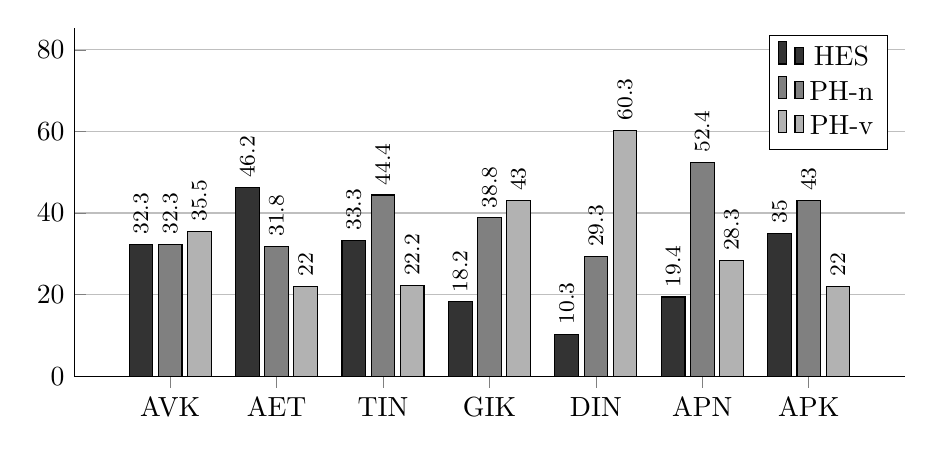
\begin{tikzpicture}
	\begin{axis}[
		ybar,
		enlarge x limits={0.15},
		enlarge y limits={abs=25,upper},
		ymajorgrids=true,
		xtick=data,
		axis lines*=left,
		ymin=0,
		nodes near coords,
		nodes near coords style={font=\footnotesize,rotate=90,anchor=west},
		width = \textwidth,
		height = 6cm,
		bar width=0.3cm,
		symbolic x coords={AVK,AET,TIN,GIK,DIN,APN,APK}
		]
		\addplot[black,fill=black!80] coordinates {(AVK,32.3) (AET,46.2) (TIN,33.3) (GIK,18.2) (DIN,10.3) (APN,19.4) (APK,35)};
		\addlegendentry{HES}
		\addplot[black,fill=black!50]
		coordinates {(AVK,32.3) (AET,31.8) (TIN,44.4) (GIK,38.8) (DIN,29.3) (APN,52.4) (APK,43)};
		\addlegendentry{PH-n}
		\addplot[black,fill=black!30] 
		coordinates {(AVK,35.5) (AET,22.0) (TIN,22.2) (GIK,43.0) (DIN,60.3) (APN,28.3) (APK,22)};
		\addlegendentry{PH-v}
	\end{axis}
	\end{tikzpicture}
\caption{Frequency of strategies of use of \textit{uŋun} by individual speakers (arranged in order of increasing proficiency), excluding unclear and indeterminate tokens as well as those that stand in for adjectives, clauses, and direct speech. Since GIKlju and LIO produced hardly any fillers, they are omitted from the figure.}
\label{fig:pakendorf:19}
\end{figure}

It is notable that with the exception of AVK all the speakers omit the target more often for verbal placeholders than for nominal placeholders (\figref{fig:pakendorf:20}). As suggested by Françoise Rose, this could be due to the fact that the verbal placeholder has a generic meaning of ‘do’ (cf. \sectref{sec:pakendorf:4.1.5}), while the nominal placeholder lacks a similar generic meaning (\sectref{sec:pakendorf:4.1.4}). This is particularly noticeable for APN, who omits the target in over 70\% of her uses of \textit{uŋun}- as a verbal placeholder, leaving it up to the hearer to reconstruct the meaning. APN also omits nominal targets very frequently (nearly 40\% of all her tokens of the filler standing in for a noun or NP lack an overt target). Possibly her advanced age – she was in her early nineties when she was recorded – made her unwilling to expend the effort needed to search for words that eluded her.

\begin{figure}
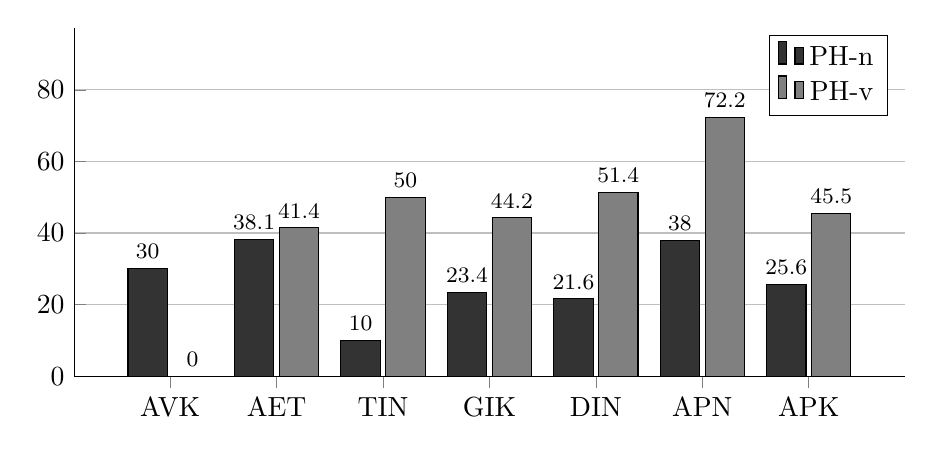
\begin{tikzpicture}
	\begin{axis}[
		ybar,
		enlarge x limits={0.15},
		enlarge y limits={abs=25,upper},
		ymajorgrids=true,
		xtick=data,
		axis lines*=left,
		ymin=0,
		nodes near coords,
		nodes near coords style={font=\footnotesize},
		width = \textwidth,
		height = 6cm,
		bar width=0.5cm,
		symbolic x coords={AVK,AET,TIN,GIK,DIN,APN,APK}
		]
		\addplot[black,fill=black!80]
		coordinates {(AVK,30.0) (AET,38.1) (TIN,10.0) (GIK,23.4) (DIN,21.6) (APN,38.0) (APK,25.6)};
		\addlegendentry{PH-n}
		\addplot[black,fill=black!50]
		coordinates {(AVK,0) (AET,41.4) (TIN,50.0) (GIK,44.2) (DIN,51.4) (APN,72.2) (APK,45.5)};
		\addlegendentry{PH-v}
		\end{axis}
	\end{tikzpicture}
 \caption{\label{fig:pakendorf:20} Proportion of placeholder uses without overt targets across speakers. GIKlju and LIO are omitted, since the extremely small number of fillers that they produced precludes meaningful analysis.}
\end{figure}

To summarize, speakers resort to using the filler with very variable frequency, and they also vary in the frequency with which they use it as a placeholder or hesitative. The choices seem to be governed by proficiency of the speakers as well as by the genre and recording context. Less proficient speakers use the filler more frequently, and in particular as a hesitative rather than as a placeholder; similarly, the pressure to narrate folk tales in a particular manner produces many fillers, especially hesitatives. In contrast, procedural texts trigger the use of targetless verbal placeholders with a generic reading.

\section{Cognitive and pragmatic aspects of filler use}
\label{sec:pakendorf:5}
\subsection{Fillers in word search}
\label{sec:pakendorf:5.1}
As mentioned in the introduction, fillers are one of the strategies speakers can use to play for time when they encounter difficulties in retrieving a lexical item. This is demonstrated particularly clearly by examples where the word search is subsequently verbalized \REF{ex:pakendorf:45}, but also by instances where a placeholder is broken off when the speaker remembers the target \REF{ex:pakendorf:46}: 


\ea \label{ex:pakendorf:45}
\gll naːndun
	man
	moː-ŋi-n
	bi-si-n
	taj
	\textup{(0)}
	\textbf{uŋun}
	\textup{(1450)}
	\textbf{uŋun}
	\textup{(1890)}
	bəjə
	moː-ŋi-nen
	taj…
	listvennica
	omŋo-ʨa
	bi-si-m\\
     \textsc{3sg.dat.ess}
     self
     tree-\textsc{poss-3sg}
     \textsc{cop-nfut-3sg}
     \textsc{dist}
     {}
     \textsc{flr}
     {}
     \textsc{flr}
     {}
     man tree-\textsc{poss-3sg}
     \textsc{dist}
     larch.R
     forget-\textsc{pst.ptcp}
     \textsc{aux-nfut-3sg}\\
\glt ‘He has his own tree [i.e. for men there is a separate tree on which to perform the holgin ritual], that \textbf{whatchamacallit/uhm}… \textbf{whatchamacallit/uhm}… A man’s tree is…. I forgot (how to say) larch [using the Russian word for ‘larch’].’ \exsource{GIK\_ostroe 20-22; ID 776-777}
\z

\ea \label{ex:pakendorf:46}
\gll taj=tti bu ɟeli-βa
	\textup{(1000)}
	\textbf{uŋun-e-β}…
	\textup{(0)}
	\uline{olo-ma-t-ʨe-βun}\\
     \textsc{dist=ptl1} \textsc{1pl.ex} taimen-\textsc{acc}
     {}
     \textsc{flr-nfut-1}
     {}
     fish-\textsc{vr-tam2-nfut-1pl.ex}\\
\glt ‘Like that we \textbf{whatchamacall…}, \uline{caught} a taimen!’ \exsource{DIN\_rybalka: 27; ID 691}
\z

Very often, when the delayed constituent is finally produced, it carries a higher pitch which emphasises it (cf. \citealt[71--73]{PodlesskayaPodlesskaya2022}, for a similar observation in Russian). This kind of emphatic pitch can follow after both hesitative uses of \textit{uŋun} and placeholder uses: in example \REF{ex:pakendorf:47}, the first token of the filler is not morphosyntactically integrated and is hence identifiable as a hesitative, with the delayed constituent \textit{bakaja} ‘they found’ pronounced with emphatic high pitch on the first syllable (\figref{fig:pakendorf:21}). The second token of the filler carries Accusative case and is clearly the placeholder for the NP \textit{ʨolʨoki samaːnman} ‘the shaman of the weasels’; this carries even higher pitch on the first syllable of \textit{ʨolʨoki} ‘weasel’. This high pitch and intensity on the delayed constituent underlines the fact for the hearer that the word search was successfully concluded.


\ea \label{ex:pakendorf:47}
\gll samaːn-a gəlɑːktə-naː-jaːn oː-mi
	\textup{(0)} \textbf{uŋun} \textup{(420)}
	baka-ja əmən
	\textup{(0)} \textbf{uŋun-ma} \textup{(660)}
	\uline{ʨolʨoki} \uline{samaːn-ma-n}\\
     shaman-\textsc{acc.indf} look.for-\textsc{am-ss.ant} make.\textsc{ss.cond}
     {} \textsc{flr} {}
     find-\textsc{nfut[3pl]} one 
     {} \textsc{flr-acc} {}
     Siberian.weasel shaman-\textsc{acc-3sg}\\
\glt ‘Having gone to look for a shaman… \textbf{uhm…} they found a \textbf{whatchamacallit}, \uline{a shaman of the Siberian weasels}.’ \exsource{APK\_frog\_tale: 120; ID 224-225}
\z

\begin{figure}
\includegraphics[clip, trim=0cm 5.9cm 0cm 2.5cm, width=\textwidth]{Fig21_224.pdf}
\caption{Waveform and pitch contour of example \REF{ex:pakendorf:47}}
\label{fig:pakendorf:21}
\end{figure}

The Negidal data partly contradict the common assumption that speakers encounter more difficulties in retrieving infrequent lexemes or items that are less predictable in a given discourse context \citep[461--462]{Lickley2015}: an admittedly rather limited analysis of the nature of the overt targets of placeholders shows that only about 40\% are items that might be considered rare,\footnote{This was estimated by checking the frequency of items in the corpus via concordance searches, but also by assuming that the names of characters in folk tales or of people who lived a long time ago would not be commonly used and hence would no longer be activated (cf. \citealt[274]{Schegloff1979}), or that the terms for archaic cultural items would be rarely used. Conversely, culturally salient items, like boats, fish hooks and lures, or the lean-to which serves as a vital storage room in houses, were considered to be common, even if they didn’t occur very frequently in the corpus. Note that when the probable delayed constituent of hesitative or indeterminate uses is included in the analysis, the relative proportions of rare vs. (very) common items remain the same.} such as names of people who lived a long time ago and whom one has hence not referred to in a while, or archaic cultural objects such as shaman’s tambourines, particular types of footwear, or the prow of birchbark boats. In contrast, nearly 39\% of the fillers are triggered by common or even very common items, sometimes on multiple occasions. For instance, ‘river/stream’, which refers to a crucial feature of the Negidal environment, occurs in the corpus 63 times and triggers a filler four times, and ‘dish/container’ (55 occurrences in the corpus) elicits a filler five times. Even some very frequent verbs, such as ‘make’ (375 occurrences in the corpus) or ‘think’ (225 occurrences in the corpus) elicit three and four fillers, respectively.

There are furthermore several instances when items that were produced in the immediately preceding context trigger the use of a placeholder, as described in \sectref{sec:pakendorf:4.1.5} for the ‘resumptive pro-verb’ use of \textit{uŋun}. Such rather unexpected uses of the filler have also been noted for the Maliseet\hyp Passamaquoddy “noun substitute” by \citet[142]{LeSourd2003}: 

\begin{quote}
 [M]any occurrences of the noun substitute do not appear to be of this character [a hesitation signal]. Often the [placeholder] pronoun is used to introduce a common word that one might expect a speaker to find easy to recall. A speaker will sometimes employ the noun substitute to introduce a noun that he or she has already used several times in a given discourse. Not surprisingly, there is often no appreciable pause in such cases before the speaker provides the target noun. We are accordingly faced with a puzzle. Why do speakers apparently use a hesitation form even when they seem to feel no need to hesitate?
\end{quote}

For example, in the sequence in \REF{ex:pakendorf:48} DIN asks her mother APN whether she remembers Tanja Trofimova’s father, but then repeats her question using the placeholder. Apart from ‘father’ being a very common word (243 instances in the corpus) that one might expect to have been easily retrievable, it was produced a mere six seconds before the placeholder, and thus might be assumed to have still been activated when DIN rephrased her question – yet it is notable that she pauses for a considerable stretch of time before the placeholder. 


\ea \label{ex:pakendorf:48}
\ea
\gll \textup{DIN:}
	siː oɲiː tanja-ŋasa trofimov-ŋasa amin-ŋasa-βa-n ɟo-ŋʨi-s\\
    ~{} \textsc{2sg} mother.\textsc{voc} \textsc{pn-dec} \textsc{pn-dec} father-\textsc{dec-acc-3sg} remember-\textsc{dur[nfut]-2sg}\\
\glt ‘Mama, do you remember the late father of late Tanja Trofimova?’ 

\ex \textup{APN:} niː?
\glt ‘Who ?’

\ex \gll \textup{DIN:}
	tanja-ŋasa
	trofimov-ŋasa
	\textup{(1530)}
	\textbf{uŋun-ma-n}
	\textup{\{}
	\textup{APN:}
	ami-nin
	\textup{\}}
	\textup{DIN:}
	\uline{amin-ma-n} ɟo-ŋʨi-s\\
	 ~{}
     \textsc{pn-dec}
     \textsc{pn-dec}
     {}
     \textsc{flr-acc-3sg}
     {}
     {}
     father-\textsc{3sg}
     {}
     {}
     father-\textsc{acc-3sg}
     remember-\textsc{dur[nfut]-2sg}\\
\glt ‘DIN: Late Tanja Trofimova’s \textbf{whatchamacallit}… \{APN: her father\} DIN: … do you remember \uline{her father}?’ \exsource{APN\_DIN\_conversation: 59-63; ID 320}
\z
\z 

In some instances, it is likely that the speakers were distracted (cf. \citealt{Lickley2015}: 463) and hence couldn’t immediately retrieve the item they needed. Unfortunately, since we lack video recordings for most of the Negidal data, it is impossible to identify external distractors, such as a bird flying by outside or a sound at the door. Nevertheless, possible causes of distraction can be identified in the data, as will be outlined in the following. These comprise 1) the presence of as-yet-unfamiliar linguists with a video camera and other recording devices, 2) the realization that one has made an error, or 3) the search for a different lexeme that is going on in the background. 

Concerning the first point, the verb \textit{uli}- ‘sew’, which appears in the corpus 110 times, elicited a placeholder on four occasions, once in an explanation of how to make thread out of elk sinew in which sewing was mentioned ten times. All tokens of the placeholder for ‘sew’ occurred in recordings done by linguists who were not yet very well known to the speakers and that involved both video and audiorecording. It is thus possible that the video camera and big audiorecorder in combination with foreign linguists facing the speakers (on one occasion, three linguists were present at the same time) distracted the speakers and led to their lack of concentration. 

As to the second type of potential distractor, it is likely that the filler in \REF{ex:pakendorf:49} was not triggered by difficulties in retrieving the word for ‘horse’, but rather by the speaker’s realization that she made a mistake (there were three horses, and not two); this may have distracted her and led to the disfluency. This is indicated by the false start on \textit{mo[jenma]} followed by a filled pause [əmm], and the fact that the filler, while carrying the appropriate Accusative suffix needed to substitute for ‘horse’, is pronounced with the low pitch and intensity found on the filled pause (\figref{fig:pakendorf:22}). In addition, there is a long pause before the numeral \textit{ɟul} ‘two’, further underlining the hesitation of the speaker. 


\ea \label{ex:pakendorf:49}
\gll alaβ-kal
	\textup{(1930)}
	ɟul
	\textup{(770)}
	mo…
	əmm
	\textbf{uŋun-ma}
	\textup{(590)}
	elan
	\uline{mojen-ma}
	gun-ə-n\\
     to.harness-\textsc{imp.sg}
     {}
     two
     {}
     \textsc{fs}
     ehm
     \textsc{flr-acc}
     {}
     three
     horse-\textsc{acc}
     say-\textsc{nfut-3sg}\\
\glt ‘“Harness two… \textbf{whatchamacallit}, three \uline{horses}”, she said.’ \exsource{TIN\_swine: 91; ID 882}
\z

\begin{figure}
\includegraphics[clip, trim=0cm 5.9cm 0cm 2.5cm, width=\textwidth]{Fig22_882.pdf}
\caption{Waveform and pitch contour of example \REF{ex:pakendorf:49}}
\label{fig:pakendorf:22}
\end{figure}

Lastly, as mentioned above, speakers might be distracted by a word search that is going on in the background. For example, in \REF{ex:pakendorf:50} the speaker, GIK, hesitates and resorts to the placeholder before producing what appears to be the target both on the basis of syntax (Accusative case) and intonation (emphatic high pitch and strong intensity), namely \textit{tomkolβa} ‘threads’ – even though the root \textit{tomko} ‘thread’ is found in the word that directly precedes the placeholder. In this case it seems as if what GIK might be struggling with is not the word ‘thread’, but rather the word for ‘rag’, as indicated by her further hesitations and the overt admission that she had forgotten the Negidal word for ‘rag’ (Russian \textit{loskuty}). She may thus have been distracted by the ongoing search for this lexeme that eluded her, triggering the unexpected placeholder for the familiar and activated term ‘thread’. 


\ea \label{ex:pakendorf:50}
\gll oː-ja-n ɟaβa-ja-n tomko-l-duki-n taj səlko-da-ββi tomko-duki-n
	\textup{(2550)} \textbf{uŋun-ma} \textup{(2370)}
	\uline{tomko-l-βa}
	\textup{(1490)} ulgə-ja-n \textup{(750)}
	taduk uŋun-ma ulgə-ja-n taj loskuty omŋut\\
     make-\textsc{nfut-3sg} take-\textsc{nfut-3sg} thread-\textsc{pl-abl-3sg} \textsc{dist} silk.thread.R-\textsc{vr-impers} thread-\textsc{abl-3sg}
     {} \textsc{flr-acc} {}
     thread-\textsc{pl-acc}
     {} to.braid-\textsc{nfut-3sg} {} then \textsc{flr-acc} to.braid-\textsc{nfut-3sg} \textsc{dist} rags.R \textsc{fs[}forget]\\
\glt ‘He first takes some of the threads, those with which one embroiders, he braids \textbf{the} \textbf{whatchamacallit}, \uline{the threads}, after that he braids the whatchamacallit, the rags - I forgot (the Negidal word).’ \exsource{GIK\_ostroe: 12; ID 771-772}
\z


Such examples indicate that the planning of an utterance is not finalized before it is begun, but continues as one speaks, and that it takes place relatively far in advance and can thus interfere with ongoing speech. They further demonstrate that it is not necessarily merely the accessibility of the target item that triggers a placeholder, but that other factors play a role as well, such as level of concentration, fatigue, physical well-being, and external and internal distractions, not all of which are easily identifiable from documentation corpora such as the one used here. Some of the factors that might have played a role in the fluctuations in filler use over time observed for the speakers APN, DIN, and GIK (\figref{fig:pakendorf:17} in \sectref{sec:pakendorf:4.2}) are: increasing familiarity with the recording linguists and hence decreasing formality of the recording situation (for the years 2005--2010), increasing age, level of tiredness and concentration at the moment of individual recordings, and particularities of the recording situation. For example, the steep increase in use of the filler observed for DIN in 2017 (\figref{fig:pakendorf:17}) might be linked to her increased age as well as to the fact that she was faced solely by unfamiliar linguists, while in the preceding years there were often several members of the family present during recording sessions.

\subsection{Fillers and utterance planning}
\label{sec:pakendorf:5.2}
The morphological integration of placeholders (\sectref{sec:pakendorf:4.1.5}) demonstrates that the syntactic outline of the utterance is planned well in advance, since inflectional morphology on the placeholder, such as case on nouns or tense suffixes and subject indexes on verbs, mirror those of the target. Mismatches in the morphology found on the placeholder and the target occur very rarely, concerning only about 3\% of the verbal placeholders and less than 6\% of the nominal placeholders. In addition, even when there are mismatches, these often involve morphemes that are semantically congruent, e.g. a Past Tense suffix on the verbal placeholder and a Non-Future marker on the target \REF{ex:pakendorf:51}, or cases with a partial overlap in functions\footnote{These involve the Locative, Dative-Essive and Allative, which can all express a goal, the Accusative instead of the Prolative, since the Accusative can occasionally express a median (as in \REF{ex:pakendorf:17} above), or the use of the unpossessed Accusative on the placeholder to mark a direct object instead of the Reflexive Possessive suffix on the target, since the latter is used to mark direct objects when the possessor is coreferential with the subject of the clause.} for the nominal placeholder \REF{ex:pakendorf:52}. In \REF{ex:pakendorf:52}, the speaker takes up the bare Allative form of the target that her sister prompts her with (indicated with curly brackets), even though she had used the possessive-marked Locative case on the placeholder.


\ea \label{ex:pakendorf:51}
\gll noŋaltin
	kogda
	iʨe-ʨa-tin
	bi
	ə-si-m
	naːn-tiki-n
	daga-ma-ja
	(1070)
	\textbf{uŋun-ʨa-l}
	(430)
	\uline{məjgɑː-ja}… \\
     \textsc{3pl}
     when.R
     see-\textsc{pst-3pl}
     \textsc{1sg}
     \textsc{neg-nfut-1sg}
     \textsc{3sg-all-3sg}
     near-\textsc{vr-neg.cvb}
     {}
     \textsc{flr-pst-pl}
     {}
     think-\textsc{nfut[3pl]}\\
\glt ‘When they saw that I am not coming to them they \textbf{did} \textbf{whatchamacallit}, \uline{they thought}….’ \exsource{GIK\_1tatarskoe: 62; ID 727}
\z


\ea \label{ex:pakendorf:52}
\gll ŋənə-m \textup{(570)} \textbf{uŋun-dula-j} \{togo-tki\} \uline{togo-tki} ŋənə-m\\
     go[\textsc{nfut]-1sg} {} \textsc{flr-loc-prfl.sg} fire-\textsc{all} fire-\textsc{all} go[\textsc{nfut]-1sg}\\
\glt ‘I go \textbf{to} \textbf{whatchamacallit}. \{To the fire.\} I go \uline{to the fire}.’ \exsource{GIK\_ojavi: 11-13; ID 762}
\z

The difference in frequency of the hesitative vs. placeholder strategies across speakers (\sectref{sec:pakendorf:4.2}) indicates that individuals have different kinds of problems with speech formulation. Even though both young and old speakers (born after 1940 and before 1925, respectively) use the placeholder strategy three times as frequently as the hesitative strategy (\tabref{tab:pakendorf:2}), there is a notable discrepancy in frequency of hesitative uses of \textit{uŋun} when comparing the less proficient speakers (AET, AVK, GIKlju, LIO) with the more proficient speakers (APK, APN, DIN, GIK, TIN). The former use the filler in its hesitative function nearly as frequently as in its placeholder function (\tabref{tab:pakendorf:2}). This is particularly pronounced for AET, as shown by \figref{fig:pakendorf:18} in \sectref{sec:pakendorf:4.2}, and contrasts strongly with the more proficient speakers, who use \textit{uŋun} as a placeholder four times more often than as a hesitative. This indicates that whereas the more proficient speakers mainly have recourse to \textit{uŋun} to fill a particular slot in an already constructed syntactic frame, the less proficient speakers have problems not only with finding particular words, but with putting the syntactic frame in place. 

\begin{table}
\begin{tabular}{lrrrr}
\lsptoprule
 & {young} & {old} & {weak} & {strong}\\
\midrule
{HES} & 24.9 & 24.2 & 42.4 & 19.9\\
{PH} & 75.1 & 75.8 & 57.6 & 80.1\\
\lspbottomrule
\end{tabular}
\caption{Comparison of hesitative vs. placeholder use by relative age and proficiency of speakers}
\label{tab:pakendorf:2}
\end{table}

\subsection{Fillers in repair}
\label{sec:pakendorf:5.3}

The Negidal filler can also be used to stall for time in order to effect a repair, as has been observed in other studies (\citealt[87]{Tree2002}, \citealt[153]{LeSourd2003}, \citealt[103]{GanenkovGanenkov2010}). However, the proportion of fillers that occur in repair contexts is quite low, as has been found cross-linguistically (\citealt[463]{Lickley2015} and references therein), involving only 5.6\% of all fillers. 

In the current language ecology of Negidal, speakers use Russian far more in their daily life than their heritage language, yet were obviously trying very hard to produce “correct” Negidal for the recordings which are, after all, intended to maintain a sample of the language for posterity. There is thus considerable pressure to avoid Russian words, as shown by the relatively frequent insertion of the filler to repair Russian lexemes (nearly 37\% of the repair contexts are of this type, cf. \REF{ex:pakendorf:53}). Yet speakers are not always successful in avoiding Russian lexemes: in nearly 17\% of occurrences of a placeholder with an overt target, that target is a Russian word \REF{ex:pakendorf:54} or an explicit search for the Negidal equivalent of a Russian term \REF{ex:pakendorf:55}. The attempt to avoid Russian lexemes is particularly striking in \REF{ex:pakendorf:30} above: after resorting to a headless relative clause to substitute for the target ‘sack’, the speaker finally gives up and uses the Russian word.


\ea \label{ex:pakendorf:53}
\gll aːji-dgi-ja-n gun(-ə-n) eːɟan eː babuʃ…
	\textup{(80)} \textbf{uŋun-mi} \textup{(140)}
	\uline{əβəka-j} ɟadga-s\\
     call-\textsc{rep-nfut-3sg} say-\textsc{nfut-3sg} \textsc{fs}[why] ehm granny.R
     {} \textsc{flr-prfl.sg} {}
     granny.\textsc{Evk-prfl.sg} swear.at[\textsc{nfut]-2sg}\\
\glt ‘He called him back and says: “Why did you insult gran… \textbf{your} \textbf{whatchamacallit}, \uline{your granny}?”’ \exsource{APN\_babulja: 41; ID 281}
\z


\ea \label{ex:pakendorf:54}
\gll nonon nonon bi sinə-βə sinə omugdə-βə-s=kəna
	\textup{(790)} \textbf{uŋuni-ktə} \textup{(800)}
	\uline{meriː-ktə} gun-ə-n\\
     previously previously \textsc{1sg} \textsc{2sg.obl-acc} \textsc{fs} belly-\textsc{acc-2sg=ptl}
     {} \textsc{flr-hort.sg} {}
     to.measure.R-\textsc{hort.sg} say-\textsc{nfut-3sg}\\
\glt ‘But first let me \textbf{whatchamacallit}, \uline{measure} your belly.’ \exsource{TIN\_old\_wolf: 46; ID 859}
\z

\ea \label{ex:pakendorf:55}
\gll oː-ja-n tudgən
	\textup{(1200)} \textbf{uŋun-duki-n} \textup{(2400)}
	ʨalban
	\textup{(480)} \textbf{uŋun-duki-n} \textup{(2700)}
	- \uline{beresta} \uline{omŋo-ʨa} \uline{bi-si-m}\\
     make-\textsc{nfut-3sg} fast.Y
     {} \textsc{flr-abl-3sg} {}
     birch
     {} \textsc{flr-abl-3sg} {}
     {} birchbark.R forget-\textsc{pst.ptcp} \textsc{aux-nfut-1sg}\\
\glt ‘He quickly made (it) \textbf{from} \textbf{whatchamacallit}, \textbf{from} birch \textbf{whatchamacallit}. - \uline{Birchbark}, I forgot (the word in Negidal).’ \exsource{AET\_burunduk: 45-46; ID 28-29}
\z

The filler is also frequently inserted when speakers correct their choice of Negidal item to a semantically more appropriate word \REF{ex:pakendorf:56} – a type of repair labelled “appropriateness-repair” by \citet[52]{Levelt1983}. Not infrequently in these cases the placeholder simply replaces the erroneous word without a more appropriate target being found \REF{ex:pakendorf:57}. 


\ea \label{ex:pakendorf:56}
\gll əsi=gdə osoki-j oje-duki-n atali-l-ʨa
	\textup{(1520)} \textbf{uŋun} \textup{(1020)}
	ɟaβa-l-ʨaː poleno-βa\\
     now=\textsc{contr} stove.\textsc{Evk-prfl.sg} top-\textsc{abl-3sg} take.off-\textsc{inch}{}-\textsc{pst[3sg]} {} \textsc{flr} {} take-\textsc{inch-pst[3sg]} log.R\\
\glt ‘Now she took off from the top of the stove… \textbf{uhm}… took a log (from the top of the stove).’ \exsource{TIN\_boy: 5; ID 847}
\z

\ea \label{ex:pakendorf:57}
\gll a naːnman suːn-ɟi sam
	\textup{(0)} \textbf{uŋun-ʨaːki-tin} \textup{(0)}
	kožanyj suːn-ɟi\\
     and.R \textsc{3sg.acc} coat-\textsc{ins} close
     {} \textsc{flr-rem.pst-3pl} {}
     leather.R coat-\textsc{ins}\\
\glt ‘And they had close… \textbf{done} \textbf{whatchamacallit} (\uline{covered}) her with a coat, a leather coat.’ \exsource{APN\_fire\_water: 60; ID 383}
\z

In \REF{ex:pakendorf:56}, the speaker first produces the word \textit{atal}-, which means ‘take off, remove’ and is used for taking off clothes, stripping bark off trees, and removing hide from a carcass; after hesitating she replaces it with \textit{ɟaβa}- ‘take, grab’, which is more appropriate for the action of taking a piece of firewood from a pile. In \REF{ex:pakendorf:57} the initially chosen verb, \textit{sam}{}-, means to close a door, while the required verb is \textit{das}{}- ‘to cover’.\footnote{The initial choice of verb in \REF{ex:pakendorf:56} is probably due to the fact that in Russian \textit{snimat’} can mean both ‘take off’ clothes and similar items as well as ‘take down’ something from above. In \REF{ex:pakendorf:57}, the initial choice of verb might have also been influenced by Russian, since the root \textit{kryt’} occurs both in \textit{zakryt’} ‘close (a door)’ and in \textit{ukryt’/pokryt’} ‘cover (with a jacket, a blanket)’.} The filler also occurs in instances of ‘factual’ repair, such as in example \REF{ex:pakendorf:49} above, where the speaker repairs the number of horses from two to three.

\subsection{Fillers in interaction}
\label{sec:pakendorf:5.4}
It has been observed in the literature (\citealt[499]{HayashiYoon2006}; cf. \citealt[146--147]{LeSourd2003}, \citealt[156--158]{Keevallik2010}) that fillers are sometimes interpreted by interlocutors as requests for help, leading to a “collaborative achievement of word search” (\citealt[499]{HayashiYoon2006}). While this kind of interaction is occasionally observed in the Negidal data (\REF{ex:pakendorf:58}, see also \REF{ex:pakendorf:48} and \REF{ex:pakendorf:52} above), it is not very frequent: only 15 out of 364 occurrences of the filler (i.e. about 4\%) in recordings in which a Negidal interlocutor was present triggered a prompt by the interlocutor.\footnote{For some texts we lack the sound files of the recordings; since I was unable to verify if there was “collaboration”, these were excluded from the count, even though some of them involved more than one Negidal speaker. Given the lack of metadata for the recordings prior to 2017, the presence of an indigenous interlocutor was assessed by whether any utterances were annotated in ELAN. This would of course miss the presence of interlocutors who didn’t say anything – so that the proportion of “collaborative achievements” cited here is an upper bound.}

\ea \label{ex:pakendorf:58}
\gll \textup{DIN:}
	nu
	i
	kuŋaːkan
	ho…	ho…
	\textup{(1100)} \textbf{uŋun-ə-n} \textup{(2800)}
	bogdi-ɟi-j
	\textup{\{}
	\textup{GIK:}
	həki-sin-ə-n
	\textup{\}}
	\uline{həki-sin-ə-n} taj taj selaβun\\
     ~{}
     \textsc{ptl.R}
     and.R
     young.human
     \textsc{fs} \textsc{fs}
     {} \textsc{flr-nfut-3sg} {}
     leg-\textsc{ins-prfl.sg}
     {}
     {}
     step.on-\textsc{tam1-nfut-3sg}
     {}
     step.on-\textsc{tam1-nfut-3sg} \textsc{dist} \textsc{dist} skewer\\
\glt ‘DIN: And a child \textbf{did} \textbf{whatchamacallit} with his foot \{GIK: stepped\} \uline{stepped} on that skewer.’ \exsource{DIN\_etal\_duck: 11-12; ID 586}
\z

This “collaboration” is not always successful, as shown by the following example \REF{ex:pakendorf:59}. Here, after APN utters the placeholder \textit{uŋunəβəj} ‘something for themselves’, her daughter prompts her with the term for ‘footwear’, which APN does not take up, using a term that none of the still living speakers knew, but that might refer to a specialized type of footwear.


\ea \label{ex:pakendorf:59}
\gll \textup{APN:}
	ili taj
	\textup{(0)} \textbf{uŋun-ə-βəj} \textup{(0)}
	paːti-ja 
	{\textup{\{}
	\textup{DIN:}}
	onta-ja-βaj
	\textup{\}}
	\textup{APN:}
	əj \uline{amusi-ja-βaj}\\
    ~{}
    or.R \textsc{dist} 
    {} \textsc{flr-dest-prfl.pl} {}
    beat.fish.skin.\textsc{Ulch-nfut[3pl]}
    {{}
    {}}
    footwear-\textsc{dest-prfl.pl}
    {}
    {}
    \textsc{prox} \textsc{?-dest-prfl.sg}\\
\glt ‘APN: Or they beat the skin \textbf{for} \textbf{whatchamacallit} \textbf{for} \textbf{themselves}. \{DIN: footwear for themselves\} For this \uline{XXX for themselves}.’ \exsource{APN\_DIN\_fish\_skin: 99-101; ID 335}
\z

In the context of interactional uses of the filler one might wonder whether recycling or its absence (cf. \sectref{sec:pakendorf:4.1.1.3}) is conditioned by the length of the pauses surrounding the filler: do speakers feel the need to “help” their interlocutor to follow the thread by repeating part or all of the material that accompanied the placeholder when they take a long time to retrieve the target? As can be seen from \tabref{tab:pakendorf:3}, this doesn’t seem to be the case: the minimal pause length is zero, i.e. absence of a pause, both before and after the filler, irrespective of whether there is recycling or not, and the maximal pause length is even longer after the filler when there is no recycling. The average and median pause length after a filler involved in recycling are a bit longer than when there is no recycling, but not substantially so. 

\begin{table}
\begin{tabular}{lrrrr}
\lsptoprule
 & \multicolumn{2}{c}{{No recycling}} & \multicolumn{2}{c}{{Recycling}}\\
& {Pause before} & {Pause after} & {Pause before} & {Pause after}\\
\midrule
{Minimum} &  0 &  0 &  0 &  0\\
{Maximum} &  2840 &  8120 &  2820 &  3660\\
{Average} &  690 &  890 &  730 & 1070\\
{Median} & 500 & 660 & 640 &  770\\
\lspbottomrule
\end{tabular}
\caption{Comparison of pause length (in milliseconds rounded to closest tens) with and without recycling}
\label{tab:pakendorf:3}
\end{table}

To summarize, the integration of placeholders demonstrates to what extent the structure of sentences is planned before they are uttered. Furthermore, even though the Negidal filler is used primarily in situations of disfluency, the data analysed here show that it is not merely the search for rare words or for Negidal alternatives of more accessible Russian words that triggers use of the filler, since \textit{uŋun} is frequently used when quite common or recently uttered words elude the speaker. The filler is also not a signal to the hearer that the speaker has difficulties in continuing her sentence, as shown by the rarity of “collaborative achievement” of word searches. This is congruent with the finding that filled pauses in English do not stand out from the speech stream and hence “…are not really compatible with the speaker intending to use the filled pause as a signal” \citep[459]{Lickley2015}. Rather, there appear to be a number of factors at play that trigger filler use, such as an ongoing search for a different lexeme or the realization that the speaker has made a mistake. Unfortunately, not all of the possible triggering factors can be elucidated with the Negidal database, since most of the recordings lack videos and detailed metadata that would let us reconstruct the external context of the speech situation.

\section{Discussion and conclusions}
\label{sec:pakendorf:6}

The current study has shown that the Negidal filler \textit{uŋun} is used very frequently in discourse, albeit with considerable variation across speakers. Although it can function both as a hesitative and a placeholder, the placeholder strategy predominates. Its primary function appears to be to gain time or to maintain the syntactic frame of the unfolding utterance in situations of disfluency, with pragmatic and interactive uses (avoidance or conspirational uses, turn-taking, and “collaborations” in word search) being absent or rare. Having only one item that can fulfill both strategies is cross-linguistically fairly common, being found in such varied languages as Negidal’s sister Evenki \citep{Klyachko2022}, Russian \citep{Podlesskaya2010}, the Caucasian languages Udi and Agul \citep{GanenkovGanenkov2010}, Amazonian Spanish \citep{Vallejos-Yopán2023}, and Tagalog \citep{Nagaya2022}. In contrast, having only one item that can substitute for both nouns and verbs is less common, either because languages have a placeholder that is used only for noun substitution, such as in Amazonian Spanish \citep{Vallejos-Yopán2023} or Udi and Agul \citep{GanenkovGanenkov2010}, or because separate forms are used to stand in for nouns and verbs, as in Nahavaq \citep{Dimock2010} and Maliseet\hyp Passamaquoddy \citep{LeSourd2003}. 

The placeholder strategy of the filler provides clear evidence that speakers plan the structure of their utterance in advance, before they retrieve the lexical items, since the placeholders carry the necessary inflectional morphology that integrates them into the frame of the sentence. That this planning is quite sophisticated is shown by the infrequent occurrence of mismatches between morphology on the placeholder and the target (see \figref{fig:pakendorf:11} in \sectref{sec:pakendorf:4.1.1.3}). As discussed above (\sectref{sec:pakendorf:5.2}), these mismatches often concern “compatible” categories, such as cases that can be used with the same function and that thus “fit into” the planned frame. These are thus formally different, but semantically and syntactically congruent. The evidence from the Negidal placeholder thus strengthens the evidence from interaction errors that has been adduced in favour of structural planning in speech production \citep[419--421]{Shattuck-Hufnagel2015}.

Several research questions have been left open and need to be addressed in the future. First of all, the current study focused mainly on the morphosyntactic aspects of the filler, with prosodic aspects being neglected; only pitch, waveform intensity, and pause length surrounding the filler were investigated (\sectref{sec:pakendorf:3}). Secondary markers of hesitation, such as lengthened final syllables of the filler itself and of preceding items were not taken into account, yet should be included in a full study of the phenomenon (cf. \citealt[458]{Lickley2015}, and references therein: “Where “fluent” silent pause is sanctioned by prosodic structure, it is likely to be preceded by a prolonged syllable […], and the same may apply to a hesitant pause […]: prolongation and silence are part of the same phenomenon”). 

Secondly, given that the hesitative strategy of \textit{uŋun} is quite infrequent, with less than 25\% of the occurrences being categorized as such (\sectref{sec:pakendorf:4.1.1.1}), an in-depth study of Negidal disfluency would be of interest: if speakers do not use \textit{uŋun} when they experience difficulties with retrieving words or with planning their further discourse, how do they hesitate? Very preliminary data based on less than 1\% of the corpus (comprising less than ten minutes of recordings from four fluent speakers) shows that the filler, including both its placeholder and its hesitative use, is about twice as frequent as other overt disfluencies, namely the hesitator \textit{əə}/\textit{ɛɛ} and the lengthening of final syllables. However, silent pauses account for {\textasciitilde}70\% of all disfluencies. These preliminary data indicate that overt, “filled” hesitation is quite rare in Negidal, but they obviously need to be confirmed with a more comprehensive study.

Furthermore, the interaction of fillers with gestures (cf. \citealt{Navaretta2015}) would be worth exploring further. The individual tokens adduced in \sectref{sec:pakendorf:3} and \sectref{sec:pakendorf:4.1.5} show interesting differences in the timing of the gesture: the pointing gesture precedes the placeholder (example \REF{ex:pakendorf:7}, \figref{fig:pakendorf:4}), while the gaze aversion follows after the hesitative (example \REF{ex:pakendorf:5}, \figref{fig:pakendorf:2}), and the rolling gesture accompanies the exophoric use of \textit{uŋun} in example \REF{ex:pakendorf:36} (\figref{fig:pakendorf:13}). It is an open question whether these distinctions are regular, and also what different kinds of gestures accompany the different uses of the filler. 

Finally, a comparison with Negidal’s sister languages might provide further interesting insights into the morphosyntactic aspects of fillers, since these languages show comparable levels of morphological complexity but use fillers of different origin. Thus, Evenki \citep{Klyachko2022} and the Bystraja dialect of Even \citep{Matić2008} have dedicated fillers (\textit{aŋi} and \textit{uŋ}, respectively), while the Lamunkhin dialect of Even makes use of interrogative proforms: \textit{iak}/\textit{ia}{}- ‘what/do what’. Preliminary data indicate that these different types of fillers might differ in how they are used, the details of which might shed more light on the diachrony and functions of fillers. 

\section*{Sources}

All the examples are taken from \citet{PakendorfAralova2017} and can be found by searching for the text ID. The numbers of annotation units are those that are found in the pdf-file of the transcribed, translated and glossed text. In ELAN files with multiple speakers it is best to choose the tier ‘phrase-segnum-en’ for the relevant speaker in the ‘Grid’ view, which provides the annotation number that corresponds to that given here.

\section*{Acknowledgements}

I thank two anonymous reviewers for their constructive comments on a first version of this chapter, and in particular Françoise Rose, whose continued discussion and constructive criticism helped me greatly improve the paper. I also thank my colleagues Jennifer Krzonowski and Rémi Anselme for assistance: Jennifer for writing the Praat script that let me automatize most of the investigation of the intonation patterns, and Rémi for providing me with the video stills shown in some figures, for help with producing images in Praat and Excel, and for ensuring that the \LaTeX~version of this chapter is free of formatting errors. The data on which this study is based were collected with the generous support of ELDP (grant MDP0346), which is gratefully acknowledged. I am also grateful to the ASLAN project (ANR-10-LABX-0081) of the Université de Lyon, for its financial support within the French program "Investments for the Future" operated by the National Research Agency (ANR). I furthermore thank Natalia Aralova for helpful discussion of the Negidal data not only while we were compiling the corpus, but also with respect to several examples of the filler. Last, but definitely not least, I thank all the Negidal speakers whom I had the pleasure to meet in person for their contributions to the corpus, and most especially DIN and GIK for their many hours of patient work on transcriptions, translations, and clarification of tricky questions.

\section*{Abbreviations used in glosses}

1, 2, 3 indicate person, \textsc{sg}, \textsc{pl} indicate singular and plural number, respectively.
\medskip


\begin{tabularx}{.45\textwidth}{lQ}
\textsc{abl} & ablative\\
\textsc{acc} & accusative\\
\textsc{acc.indf} & indefinite accusative\\
\textsc{add} & additive\\
\textsc{advb.all} & adverbial allative\\
\textsc{advr} & adverbializer\\
\textsc{all} & allative\\
\textsc{am} & associated motion\\
\textsc{aux} & auxiliary\\
\textsc{caus} & causative\\
\textsc{cond} & conditional\\
\textsc{contr} & contrastive\\
\textsc{cop} & copula\\
\textsc{dat.ess} & dative-essive\\
\textsc{dec} & decessive (refers to deceased people)\\
\textsc{deont} & deontic future\\
\textsc{dest} & destinative\\
\textsc{dim} & diminutive\\
\textsc{dist}  & distal demonstrative\\
\textsc{dp} & discourse particle\\
\textsc{dur} & durative\\
\textsc{euph} & euphemism\\
\textsc{Evk} & Evenki borrowing\\
\end{tabularx}
\begin{tabularx}{.45\textwidth}{lQ}
\textsc{ex} & exclusive\\
\textsc{flr} & filler\\
\textsc{foc} & focus\\
\textsc{fs} & false start\\
\textsc{hab} & habitual aspect\\
\textsc{hab.ptcp} & habitual participle\\
\textsc{hort} & hortative (1st person imperative)\\
\textsc{ideo} & ideophone\\
\textsc{imp} & immediate future imperative (2nd person)\\
\textsc{impers} & impersonal\\
\textsc{inch} & inchoative \\
\textsc{ins} & instrumental\\
\textsc{interj} & interjection\\
\textsc{intr} & intransitive\\
\textsc{ints} & intensive\\
\textsc{ints.adj} & intensive adjectivizer\\
\textsc{iter} & iterative\\
\textsc{loc} & locative\\
\textsc{mult} & multiplicative\\
\textsc{neg} & negative auxiliary\\
\end{tabularx}


\begin{tabularx}{.45\textwidth}{lQ}
\textsc{neg.cvb} & negative converb\\
\textsc{neg.fut} & future tense suffix restricted to negative auxiliary\\
\textsc{nfut} & non-future\\
\textsc{Nnc} & borrowing from a Nanaic language \\
\textsc{num(days)} & numeral derivation expressing number of days\\
\textsc{obl} & oblique\\
\textsc{pass.ptcp} & passive participle\\
\textsc{pl.hum} & plural of nouns designating humans\\
\textsc{pn} & personal name\\
\textsc{poss} & marker of non-canonical possessive construction\\
\textsc{prfl} & reflexive possessive\\
\textsc{prol} & prolative\\
\textsc{prox} & proximal demonstrative\\
\textsc{prs.ptcp} & present participle\\
\textsc{pst} & past tense\\
\textsc{pst.ptcp} & past participle\\
\textsc{ptl} & particle\\
\textsc{q.fut} & interrogative future\\
R & Russian borrowing\\
\textsc{rem.pst} & remote past\\
\textsc{rem.ptcp} & remote participle\\
\end{tabularx}
\begin{tabularx}{.45\textwidth}{lQ}
\textsc{rep} & refactive (repeated action)\\
\textsc{res} & resultative\\
\textsc{restr} & restrictive\\
\textsc{side} & derivative suffix with a meaning of ‘side’\\
\textsc{sml} & similative\\
\textsc{smlf} & semelfactive\\
\textsc{ss.ant} & same-subject anterior converb\\
\textsc{ss.cond} & same-subject conditional converb\\
\textsc{ss.dur} & same-subject durative converb\\
\textsc{ss.sim} & same-subject simultaneous converb\\
\textsc{sudden} & sudden action\\
\textsc{tam} & tense-aspect-mood marker\\
\textsc{tr}  & transitive\\
\textsc{Ulch} & Ulch borrowing\\
\textsc{val} & valency-changing suffix\\
\textsc{voc} & vocative\\
\textsc{vr} & verbalizer\\
\textsc{vs.purp} & variable-subject purposive converb\\
\textsc{vs.sim} & variable-subject simultaneous converb\\
Y & Sakha (Yakut) borrowing\\
\\
\end{tabularx}

\sloppy\printbibliography[heading=subbibliography,notkeyword=this]
\end{document} 
